\documentclass[10pt,a4paper]{article}
\usepackage[utf8]{inputenc}
\usepackage[T1]{fontenc}
\usepackage[spanish,es-nodecimaldot]{babel}
\usepackage[margin=2cm]{geometry}
\usepackage{graphicx}
\usepackage{amsmath}
\usepackage{float}
\usepackage{longtable}
\usepackage{microtype}
\usepackage[colorlinks=true,urlcolor=blue,linkcolor=blue]{hyperref}
\setlength{\parindent}{0pt}
\setlength{\parskip}{5pt}
\begin{document}
\begin{center}
{\Large\bfseries Cuenca del río La Vieja}\\[3pt]
{\large Exploración hidroclimática mensual}\\[5pt]
Curso de Hidrología -- Tarea 1\\
{\small Documento en construcción -- Orden de la guía}
\end{center}
\tableofcontents
\clearpage
\section*{Introducción}
Pendiente de redacción final.
\section*{Metodología}
Los procedimientos existentes se conservan junto a cada análisis; la metodología integrada está pendiente de redacción final.
\section*{Resultados y discusión física}

\section*{Contexto geográfico de la cuenca}
\subsubsection*{Contexto geográfico con base cartográfica}
Además del mapa analítico sin teselas, se incluye una versión geográfica con
base OpenStreetMap. Muestra el polígono de cuenca, las estaciones activas de
lluvia y Cartago. La base es únicamente contexto cartográfico; no se usa para
calcular resultados. Fuente de la base: © OpenStreetMap contributors.
\begin{figure}[H]\centering
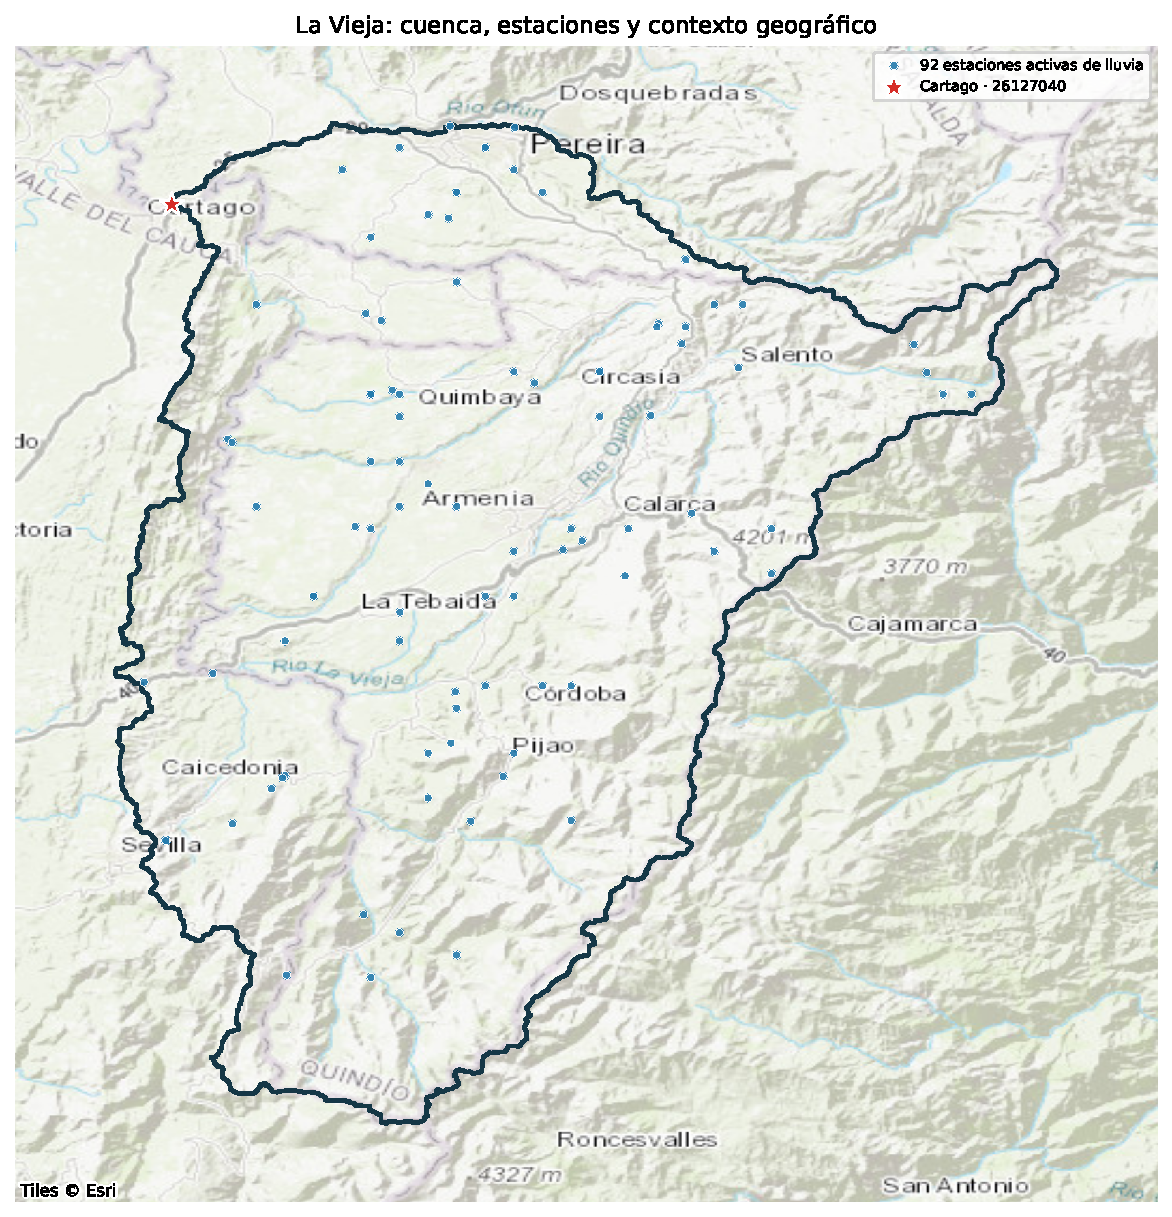
\includegraphics[width=.82\linewidth]{figuras/mapa_cuenca_estaciones_geografico.pdf}
\caption{Cuenca La Vieja, estaciones de lluvia inventariadas y estación Cartago sobre contexto geográfico OpenStreetMap.}
\end{figure}

\clearpage
\subsubsection*{Mapas de la cuenca y topografía}
\subsubsection*{Delimitación y red terrestre inventariada}
Se utiliza el polígono CAMELS transformado a WGS84 y la ubicación de Cartago del
catálogo IDEAM. Los 92 puntos son estaciones activas de categorías que miden
lluvia; no se ha verificado la continuidad de sus series.
\begin{figure}[H]\centering
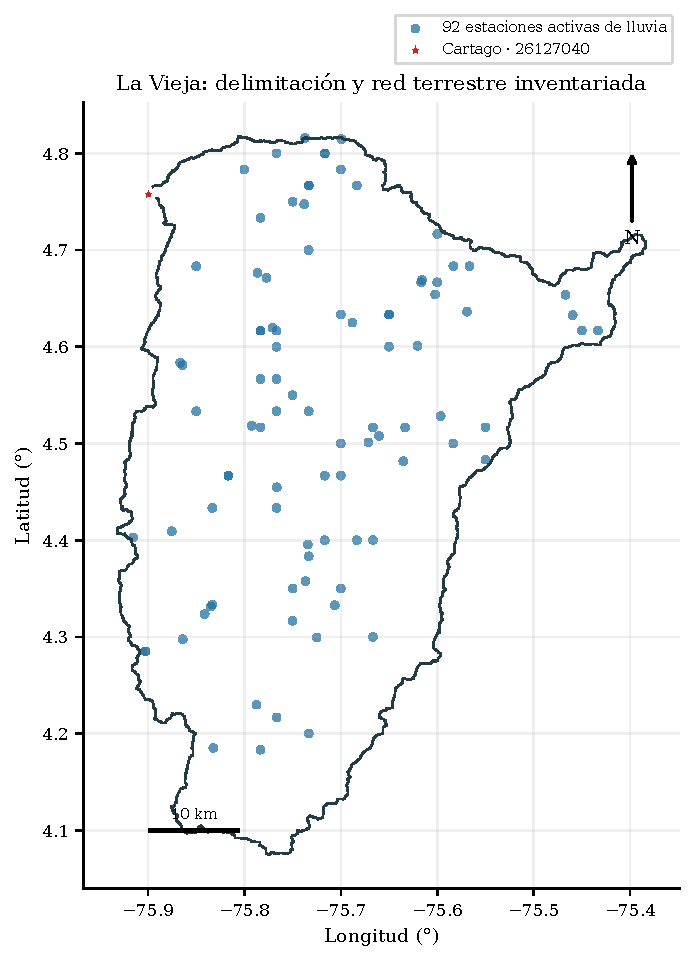
\includegraphics[width=.72\linewidth]{figuras/mapa_cuenca_estaciones.pdf}
\caption{Cuenca La Vieja hasta Cartago y estaciones terrestres inventariadas.}
\end{figure}

\subsubsection*{Modelo de elevación descargado}
Se descargó Copernicus DEM GLO-30 público, mosaico N04/W076, y se recortó al
polígono. Se conserva el GeoTIFF a resolución nominal de unos 30 m; la figura
usa una malla reducida por promedio. Es un modelo de superficie (DSM), que puede
incluir vegetación y construcciones, no un modelo de terreno desnudo.
\begin{figure}[H]\centering
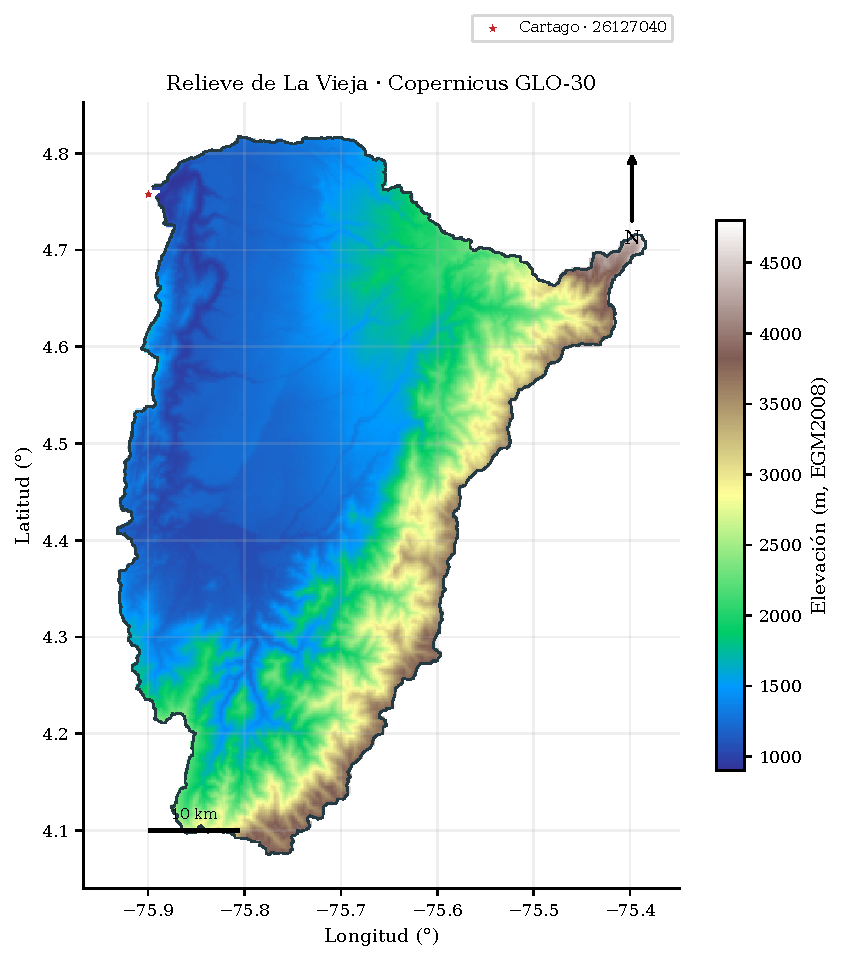
\includegraphics[width=.72\linewidth]{figuras/mapa_relieve.pdf}
\caption{Relieve de La Vieja con Copernicus GLO-30. Alturas en metros, EGM2008.}
\end{figure}
El recorte presenta mínimo 908.5 m, media de píxeles 1799.0 m y máximo 4774.2 m. 
CAMELS reporta 940,54, 1826,21 y 4795 m, respectivamente. Las diferencias entre
modelos, máscaras y resolución se documentan y no sustituyen automáticamente los
atributos originales. El DSM no representa cambios durante el periodo 1981--2022.

Fuente: \href{https://doi.org/10.5270/ESA-c5d3d65}{Copernicus DEM} y
\href{https://copernicus-dem-30m.s3.amazonaws.com/readme.html}{distribución pública COG}.

{\footnotesize produced using Copernicus WorldDEM-30 \textcopyright\ DLR e.V.
2010-2014 and \textcopyright\ Airbus Defence and Space GmbH 2014-2018 provided
under COPERNICUS by the European Union and ESA; all rights reserved}

\clearpage
\section{Series mensuales: exploración y validación}

\subsection{Graficar las series de caudal y precipitación}
\subsubsection*{Series de precipitación y caudal}

Se analiza la cuenca del río La Vieja hasta la estación Cartago (IDEAM 26127040), con un área CAMELS de 2797,19~km$^2$. El periodo comprende enero de 1981 a diciembre de 2022. Se utiliza precipitación CHIRPS v2 promediada sobre la cuenca y caudal observado según el depósito \href{https://doi.org/10.5281/zenodo.18794895}{CAMELS-COL}.

Para mantener una notación explícita, $P_{L,m}$ es la precipitación de referencia elegida: CHIRPS v2 diario, promediado sobre la cuenca por CAMELS-COL y acumulado a mm/mes. CHIRPS es un producto combinado espacial, no la observación independiente de un único pluviómetro local. $P_{I,m}$ es IMERG Final Run V07 en mm/mes. Para la comparación simultánea de $P_{L,m}$, $P_{I,m}$ y Q se define enero de 1998--diciembre de 2022, con 285 meses completos; los 15 meses sin Q se mantienen como faltantes y no se rellenan.

\subsubsection*{Agregación y tratamiento de faltantes}
La precipitación mensual se obtiene sumando los valores diarios y el caudal mensual promediándolos. Para un mes completo con $n_m$ días:
\[
P_m=\sum_{d\in m}P_d\quad[\mathrm{mm/mes}],\qquad
Q_m=\frac{1}{n_m}\sum_{d\in m}Q_d\quad[\mathrm{m^3/s}].
\]
Se conserva únicamente un mes con el 100\,\% de sus días válidos. El calendario contiene 15\,340 días esperados y 255 ausentes (1,66\,\%). Quedan 485 meses completos de 504; los 19 restantes se mantienen como vacíos. No se rellenan ni prorratean registros y se conservan los extremos.

\begin{figure}[H]
\centering
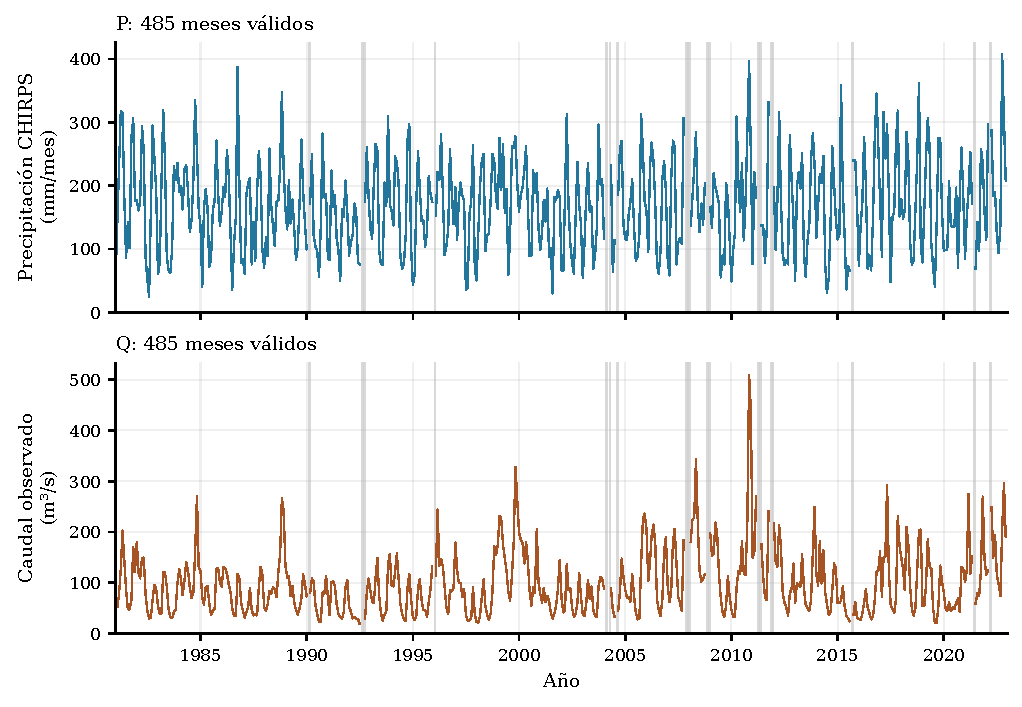
\includegraphics[width=\linewidth]{figuras/series_mensuales.pdf}
\caption{Precipitación acumulada y caudal medio mensuales de La Vieja--Cartago. Los paneles comparten el eje temporal; las franjas grises indican meses excluidos por días faltantes. Elaboración propia con CAMELS-COL.}
\label{fig:series-mensuales}
\end{figure}

\subsubsection*{Lectura inicial y alcance}
Se observan oscilaciones estacionales y diferencias entre años (figura~\ref{fig:series-mensuales}). El máximo de precipitación mensual ocurre en octubre de 2022 (407,57~mm); el máximo de caudal medio mensual, en noviembre de 2010 (508,77~m$^3$/s). No coinciden, lo que motiva examinar los aportes previos y la respuesta de la cuenca sin atribuir todavía una causa.

\subsubsection*{Meses extremos y contraste cronológico}
Los extremos que deben localizarse en la figura~\ref{fig:series-mensuales} son: agosto de 1982, mínimo de P (24,89~mm); octubre de 2022, máximo de P (407,57~mm); julio de 1992, mínimo de Q (18,37~m$^3$/s) y R (17,59~mm); y noviembre de 2010, máximo de Q (508,77~m$^3$/s) y R (471,45~mm). R es una conversión del caudal a lámina mensual, por lo cual sus extremos son coherentes con los de Q.

Que el máximo de P y el de Q ocurran en meses distintos no indica por sí solo un error: el caudal integra lluvia antecedente, almacenamiento y respuesta de la cuenca. Noviembre de 2010 es un episodio plausible: IDEAM documentó una temporada lluviosa inusitada durante La Niña, con humedad del suelo superior a la usual e inundaciones en las regiones Andina y del Cauca. Los mínimos de 1982 y 1992 también son compatibles con periodos secos asociados a El Niño reportados por IDEAM. Esta interpretación es de plausibilidad, no de causalidad: aún se deben revisar datos diarios, metadatos y cambios de instrumento para descartar un problema de medición.

\subsubsection*{Referencias del contraste climático}
IDEAM (2010). \textit{Boletín diciembre de 2010}. Disponible en \url{https://www.ideam.gov.co/file-download/download/public/6150}.

IDEAM (2006). \textit{La sequía en Colombia}, nota técnica NT\_IDEAM-2006-004.

Esta primera sección presenta las series históricas y la comparación IMERG disponible desde 1998. Las gráficas no demuestran por sí solas tendencias ni causas físicas. El código Python genera la figura vectorial y una versión Plotly con las mismas fechas y valores para su exploración interactiva.\subsubsection*{Temperatura mensual}
Se grafican las medias mensuales de Tmin y Tmax diarias de MSWX incluidas en
CAMELS, no los extremos absolutos del mes. La \textbf{temperatura media es estimada}:
$T_{d,\mathrm{est}}=(T_{d,\min}+T_{d,\max})/2$, seguida del promedio mensual.
No equivale necesariamente a una media de observaciones horarias. Se conservan
485 meses completos por curva y se mantienen los vacíos.
\begin{figure}[H]\centering
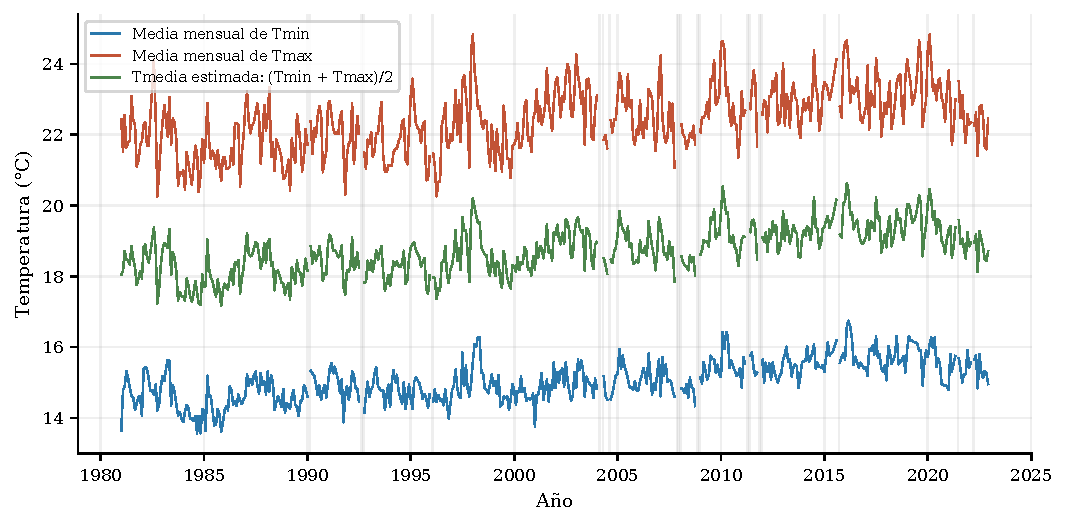
\includegraphics[width=\linewidth]{figuras/temperaturas_mensuales.pdf}
\caption{Medias mensuales de Tmin, Tmax y temperatura media estimada de la cuenca.}
\end{figure}


\subsubsection*{Temperatura media mensual directa: ERA5-Land}
Se incorporó la variable temperatura del aire a 2 m (	exttt{t2m}) del producto
ERA5-Land monthly averaged data. Es un reanálisis y no una medición puntual de
estación. La variable se descargó en kelvin y se convirtió como
$T~(^{\circ}\mathrm{C})=T~(\mathrm{K})-273,15$.

Se usa enero de 1981--diciembre de 2022: 504 meses completos, sin faltantes.
La descarga tiene malla regular de $0,1^\circ$; se intersectaron 36 celdas con
el polígono de la cuenca y se aplicó un promedio ponderado por área de
intersección. La cobertura del polígono fue 100.0\,\%. Esta serie se conserva
separada de Tmin/Tmax MSWX y de la Tmedia estimada; en adelante se usa ERA5-Land
para la temperatura media mensual.
\begin{figure}[H]\centering
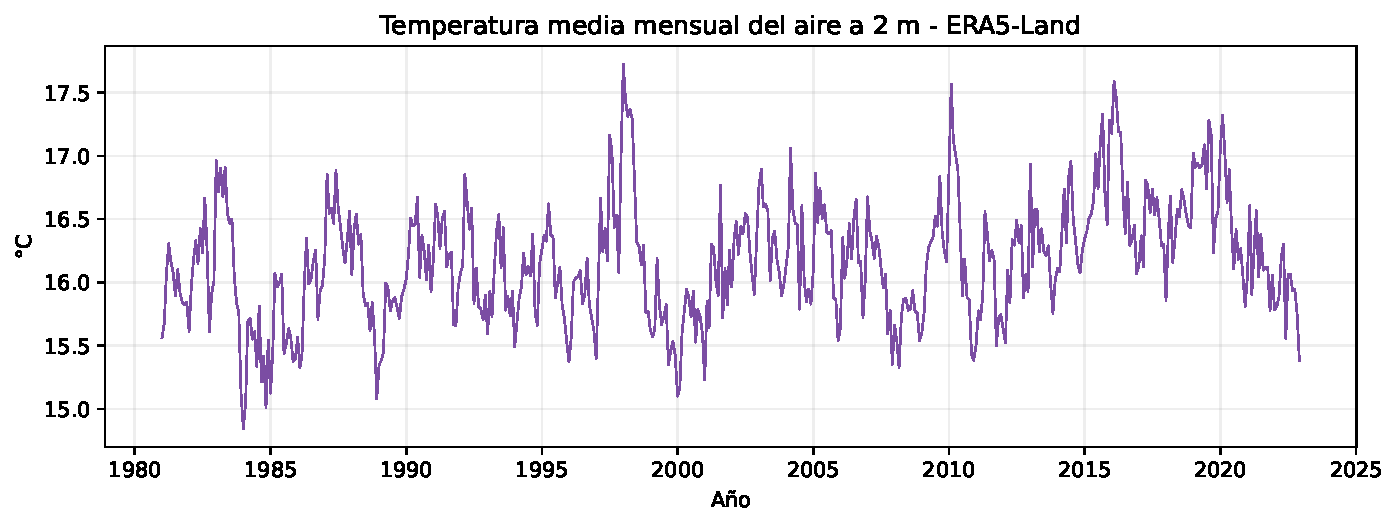
\includegraphics[width=\linewidth]{figuras/era5_land_t2m_mensual.pdf}
\caption{Temperatura media mensual del aire a 2 m de ERA5-Land, promedio ponderado sobre la cuenca de La Vieja, 1981--2022.}
\end{figure}

\subsubsection*{Agregación mensual, escorrentía y temperatura}
Para meses completos, con $P_d$ como precipitación diaria en mm, $Q_d$ como caudal medio diario en m$^3$/s y $n_m$ como número de días del mes, se usan
\[
P_m=\sum_{d\in m}P_d,\qquad \overline{Q}_m=\frac{1}{n_m}\sum_{d\in m}Q_d.
\]
Para comparar precipitación y escorrentía en láminas equivalentes, el caudal diario se convierte con el área de drenaje $A=2797,19$~km$^2$:
\[
R_m=\frac{86,4}{A}\sum_{d\in m}Q_d\quad [\mathrm{{mm/mes}}].
\]
La serie R del informe ya se calculó con esa expresión; por tanto no es una observación independiente de Q. No se debe repetir la conversión por área si el caudal ya estuviera expresado como lámina diaria.

La fuente original disponible contiene Tmin y Tmax diarios de MSWX, pero no una temperatura media directamente observada. Se grafica de manera provisional $T_{\mathrm{media,est}}=(T_{\min}+T_{\max})/2$, identificada como estimada. No se presenta como ERA5-Land/ERA5 ni como observación directa; debe contrastarse o reemplazarse con una fuente de temperatura media directa antes de una interpretación climática final.

\begin{figure}[H]\centering
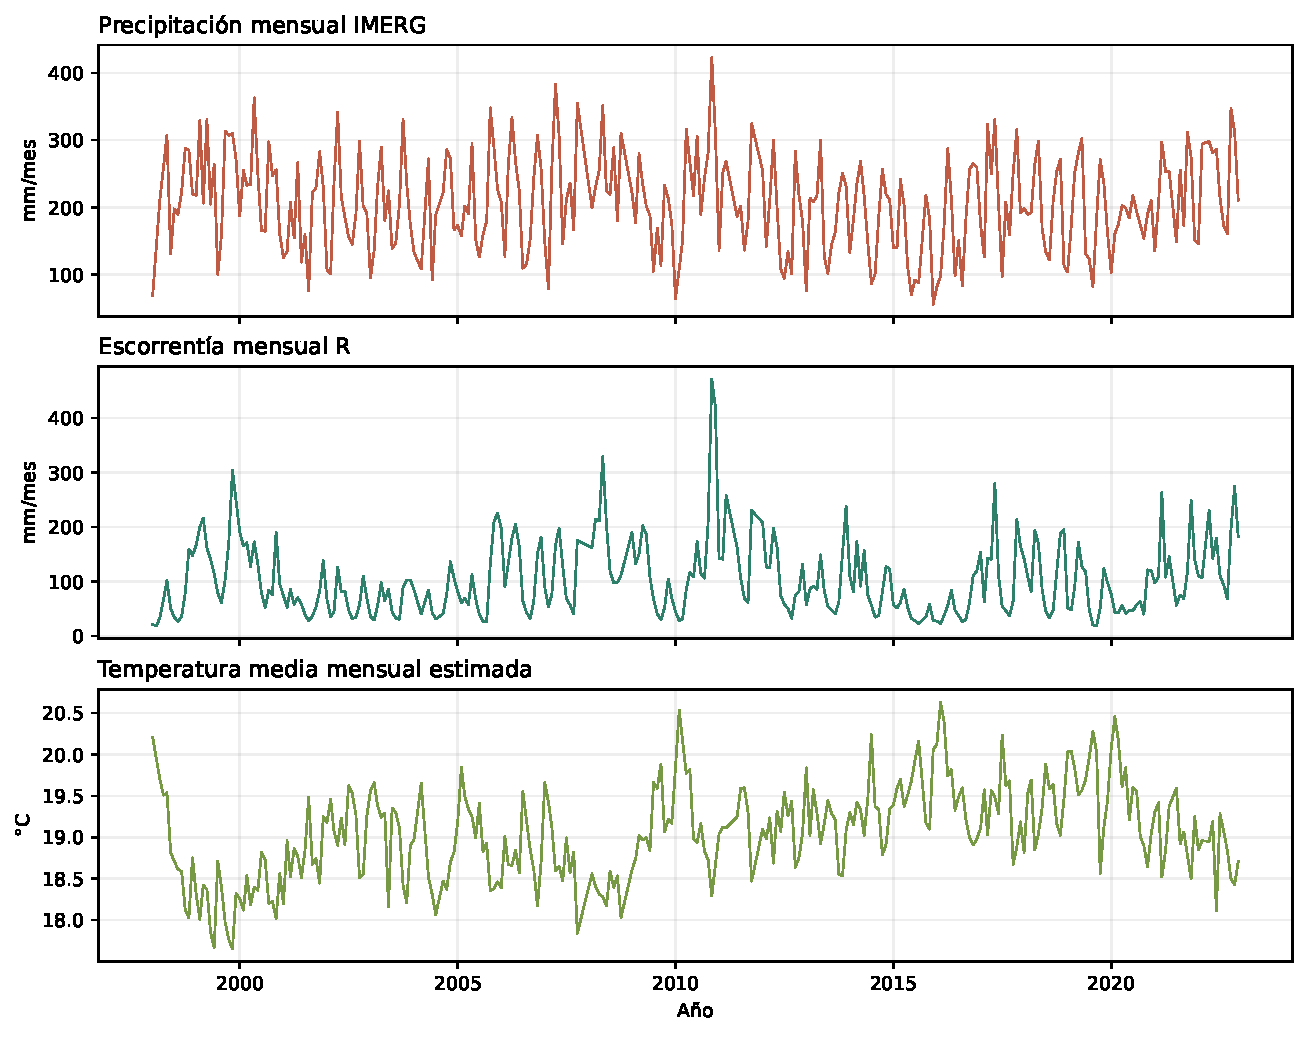
\includegraphics[width=\linewidth]{figuras/imerg_r_temperatura_comun.pdf}
\caption{IMERG, escorrentía mensual R y temperatura media mensual estimada, para los 285 meses completos simultáneos. IMERG y R están en mm/mes.}
\end{figure}



\subsection{Incorporar precipitación IMERG para la misma cuenca}


El máximo mensual de IMERG es noviembre de 2008 (431,15~mm/mes), pero Q no está disponible ese mes; se conserva la lluvia y no se inventa caudal. El mínimo es diciembre de 2015 (56,10~mm/mes; Q=29,70~m$^3$/s). Con P25=152,59 y P75=262,82~mm/mes, el episodio seco más persistente es mayo--septiembre de 2015 (cinco meses, media 98,86~mm/mes), mientras el húmedo más persistente es febrero--junio de 2022 (cinco meses, media 293,36~mm/mes).

Los años con mayor precipitación media IMERG son 2008, 2011 y 2022, y 2015 es el más seco; son contrastes aparentes entre años, no una tendencia demostrada. En los 285 meses simultáneos, la correlación IMERG--Q es 0,63; con IMERG retrasado un mes es 0,61 y con dos meses 0,32. La asociación parece concentrarse en el mismo mes o en una escala menor que un mes, pero no identifica causalidad ni separa el efecto de almacenamiento, regulación y ciclo anual compartido.



\subsection{Describir la distribución de los datos mensuales}
\subsubsection*{Periodo de datos y estadística descriptiva}
Los registros originales son diarios y se agregaron a escala mensual. El periodo
comprende enero de 1981 a diciembre de 2022 (42 años). Se describen los valores
mensuales válidos de precipitación acumulada y caudal medio, no los registros
diarios ni los totales anuales.

En las tablas, P corresponde a precipitación en mm/mes y Q a caudal en m$^3$/s.
Se usa desviación estándar muestral ($n-1$ en el denominador), mediana con
interpolación lineal y media aritmética de meses válidos. La media global no es
la media de medias anuales ni un promedio ponderado por la duración del mes.

\subsubsection*{Periodo completo: 1981--2022}
\begin{center}\small
\begin{tabular}{llrrrrrr}\hline
Periodo & Variable & Meses & Media & Mediana & Desv. est. & Mínimo & Máximo \\
\hline
1981--2022 & P & 485 & 168,20 & 168,47 & 74,54 & 24,89 & 407,57 \\
1981--2022 & Q & 485 & 98,70 & 85,55 & 64,35 & 18,37 & 508,77 \\
\hline\end{tabular}\end{center}
Los mínimos y máximos son extremos de valores mensuales. En Q, la media superior
a la mediana refleja la influencia de meses de caudal alto. La desviación estándar
describe dispersión, no error de medición.

\subsubsection*{Descripción por año}
Se indica el número de meses válidos en cada año. Si es menor de 12, las cifras
describen únicamente los meses disponibles. Los años incompletos no representan
todo el ciclo anual y su comparación puede verse afectada por los meses ausentes.
No se rellenaron datos. Todos los valores conservan las unidades mensuales indicadas.

\begingroup\small
\begin{longtable}{llrrrrrr}
\caption{Estadística por año de las series mensuales válidas. P: mm/mes; Q: m$^3$/s.}\\
\hline
Periodo & Variable & Meses & Media & Mediana & Desv. est. & Mínimo & Máximo \\
\hline\endfirsthead
\multicolumn{8}{l}{Continuación: estadística de valores mensuales por año}\\
\hline
Periodo & Variable & Meses & Media & Mediana & Desv. est. & Mínimo & Máximo \\
\hline\endhead
\hline\multicolumn{8}{r}{Continúa en la siguiente página}\\\endfoot
\hline\endlastfoot
1981 & P & 12 & 193,75 & 178,14 & 93,67 & 50,94 & 317,79 \\
1981 & Q & 12 & 99,67 & 80,62 & 52,06 & 47,08 & 202,46 \\
1982 & P & 12 & 177,36 & 176,65 & 88,06 & 24,89 & 295,10 \\
1982 & Q & 12 & 94,94 & 91,52 & 48,41 & 29,20 & 179,60 \\
1983 & P & 12 & 157,73 & 150,50 & 90,59 & 60,53 & 319,78 \\
1983 & Q & 12 & 63,58 & 47,39 & 34,47 & 29,81 & 121,33 \\
1984 & P & 12 & 203,15 & 195,19 & 55,62 & 127,90 & 335,22 \\
1984 & Q & 12 & 123,51 & 115,19 & 54,09 & 69,79 & 270,65 \\
1985 & P & 12 & 149,21 & 162,07 & 61,77 & 40,85 & 271,16 \\
1985 & Q & 12 & 81,44 & 80,09 & 33,68 & 36,39 & 128,91 \\
1986 & P & 12 & 174,99 & 171,39 & 91,02 & 36,16 & 387,11 \\
1986 & Q & 12 & 87,50 & 94,53 & 35,42 & 33,61 & 130,94 \\
1987 & P & 12 & 150,55 & 164,41 & 67,31 & 61,08 & 254,17 \\
1987 & Q & 12 & 62,67 & 45,31 & 34,82 & 31,18 & 130,72 \\
1988 & P & 12 & 175,37 & 172,47 & 79,72 & 70,59 & 347,59 \\
1988 & Q & 12 & 112,18 & 85,60 & 73,03 & 44,06 & 267,05 \\
1989 & P & 12 & 159,96 & 152,72 & 50,58 & 82,62 & 272,84 \\
1989 & Q & 12 & 83,15 & 83,46 & 31,74 & 36,50 & 133,88 \\
1990 & P & 11 & 153,48 & 135,66 & 68,54 & 56,98 & 282,22 \\
1990 & Q & 11 & 70,30 & 78,68 & 32,31 & 21,79 & 113,63 \\
1991 & P & 12 & 140,57 & 153,74 & 54,08 & 49,89 & 224,02 \\
1991 & Q & 12 & 66,58 & 64,13 & 30,72 & 28,22 & 104,98 \\
1992 & P & 10 & 142,64 & 140,27 & 57,98 & 75,46 & 260,56 \\
1992 & Q & 10 & 44,98 & 30,77 & 28,54 & 18,37 & 108,17 \\
1993 & P & 12 & 173,01 & 169,04 & 77,33 & 74,72 & 309,60 \\
1993 & Q & 12 & 81,32 & 68,11 & 46,05 & 24,98 & 156,03 \\
1994 & P & 12 & 168,17 & 149,09 & 80,53 & 69,16 & 297,40 \\
1994 & Q & 12 & 82,94 & 90,81 & 40,66 & 24,71 & 157,55 \\
1995 & P & 12 & 151,82 & 159,00 & 61,41 & 43,70 & 253,92 \\
1995 & Q & 12 & 63,31 & 54,09 & 33,97 & 25,79 & 132,32 \\
1996 & P & 11 & 178,94 & 188,43 & 60,95 & 90,85 & 281,15 \\
1996 & Q & 11 & 109,54 & 90,67 & 55,85 & 38,47 & 243,89 \\
1997 & P & 12 & 149,50 & 175,82 & 70,46 & 36,10 & 264,49 \\
1997 & Q & 12 & 75,66 & 79,35 & 47,51 & 24,65 & 179,15 \\
1998 & P & 12 & 171,40 & 180,08 & 67,09 & 50,72 & 250,25 \\
1998 & Q & 12 & 68,39 & 46,61 & 51,47 & 21,34 & 172,37 \\
1999 & P & 12 & 202,95 & 199,53 & 68,92 & 59,15 & 277,91 \\
1999 & Q & 12 & 175,34 & 174,11 & 76,98 & 64,06 & 328,46 \\
2000 & P & 12 & 178,51 & 187,12 & 53,78 & 89,25 & 262,68 \\
2000 & Q & 12 & 136,35 & 139,77 & 53,14 & 54,43 & 205,94 \\
2001 & P & 12 & 141,41 & 160,47 & 52,57 & 30,12 & 195,59 \\
2001 & Q & 12 & 68,81 & 62,85 & 30,52 & 29,21 & 144,92 \\
2002 & P & 12 & 145,48 & 145,84 & 76,41 & 61,77 & 312,58 \\
2002 & Q & 12 & 70,04 & 64,94 & 32,66 & 33,17 & 136,76 \\
2003 & P & 12 & 159,29 & 163,11 & 71,63 & 54,71 & 296,50 \\
2003 & Q & 12 & 68,48 & 62,52 & 31,76 & 33,21 & 111,06 \\
2004 & P & 9 & 163,95 & 138,10 & 75,56 & 63,98 & 270,65 \\
2004 & Q & 9 & 75,72 & 80,57 & 38,03 & 32,69 & 147,37 \\
2005 & P & 12 & 161,74 & 144,76 & 69,08 & 81,69 & 312,95 \\
2005 & Q & 12 & 98,20 & 72,59 & 69,81 & 27,63 & 236,02 \\
2006 & P & 12 & 169,88 & 182,09 & 71,71 & 60,99 & 268,06 \\
2006 & Q & 12 & 133,44 & 150,54 & 66,60 & 34,53 & 214,67 \\
2007 & P & 10 & 160,20 & 113,47 & 92,29 & 58,10 & 306,24 \\
2007 & Q & 10 & 111,81 & 86,58 & 59,89 & 43,54 & 206,06 \\
2008 & P & 9 & 182,40 & 171,76 & 50,22 & 127,33 & 284,31 \\
2008 & Q & 9 & 183,04 & 180,70 & 80,22 & 102,04 & 344,13 \\
2009 & P & 12 & 149,60 & 168,52 & 54,26 & 55,40 & 219,60 \\
2009 & Q & 12 & 118,63 & 114,71 & 65,09 & 32,35 & 218,37 \\
2010 & P & 12 & 200,31 & 189,70 & 100,31 & 48,77 & 396,03 \\
2010 & Q & 12 & 168,51 & 118,32 & 153,65 & 32,17 & 508,77 \\
2011 & P & 8 & 161,89 & 137,53 & 83,81 & 76,16 & 332,02 \\
2011 & Q & 8 & 155,98 & 156,00 & 73,42 & 65,67 & 270,32 \\
2012 & P & 12 & 161,07 & 162,50 & 80,71 & 75,31 & 315,42 \\
2012 & Q & 12 & 117,27 & 109,85 & 61,26 & 34,73 & 217,76 \\
2013 & P & 12 & 172,80 & 197,02 & 79,74 & 50,50 & 282,71 \\
2013 & Q & 12 & 101,73 & 90,72 & 60,29 & 43,71 & 249,11 \\
2014 & P & 12 & 156,19 & 161,32 & 75,40 & 30,97 & 262,57 \\
2014 & Q & 12 & 101,66 & 96,20 & 45,67 & 36,19 & 181,35 \\
2015 & P & 11 & 157,95 & 122,87 & 94,88 & 36,47 & 359,33 \\
2015 & Q & 11 & 49,82 & 54,16 & 20,74 & 23,97 & 92,77 \\
2016 & P & 12 & 176,60 & 161,45 & 95,37 & 66,46 & 345,40 \\
2016 & Q & 12 & 58,55 & 45,10 & 34,97 & 25,74 & 124,10 \\
2017 & P & 12 & 200,29 & 180,52 & 88,86 & 47,84 & 318,55 \\
2017 & Q & 12 & 130,35 & 134,80 & 78,59 & 40,39 & 292,92 \\
2018 & P & 12 & 180,37 & 165,50 & 87,41 & 75,46 & 362,47 \\
2018 & Q & 12 & 125,05 & 123,58 & 63,95 & 34,91 & 209,59 \\
2019 & P & 12 & 177,86 & 164,75 & 91,98 & 40,56 & 307,06 \\
2019 & Q & 12 & 85,95 & 74,89 & 51,64 & 20,33 & 186,15 \\
2020 & P & 12 & 150,42 & 136,46 & 56,12 & 71,11 & 260,05 \\
2020 & Q & 12 & 67,11 & 55,33 & 30,91 & 42,01 & 131,09 \\
2021 & P & 11 & 165,21 & 159,92 & 65,78 & 68,52 & 258,27 \\
2021 & Q & 11 & 138,36 & 122,42 & 72,35 & 58,91 & 275,02 \\
2022 & P & 11 & 213,48 & 190,40 & 98,93 & 93,92 & 407,57 \\
2022 & Q & 11 & 164,50 & 148,99 & 68,53 & 73,93 & 296,50 \\
\end{longtable}\endgroup
\subsubsection*{Histogramas y estadísticos completos}
Periodo: enero de 1981--diciembre de 2022. Se utilizan 485 meses completos por
variable; se excluyen 19 con faltantes, sin rellenos, prorrateos ni eliminación
automática de extremos. Se conservan los ceros. Se reúnen meses de distintas
estaciones del año, no la variabilidad de un único mes calendario.

P es precipitación CHIRPS acumulada (mm/mes); Q, caudal medio (m$^3$/s);
R, lámina de escorrentía (mm/mes). Se convierte con
$R_m=(86.4/2797.19)\sum Q_d$. R no es una observación independiente de Q.
Tmin/Tmax son medias mensuales de extremos diarios MSWX y Tmedia es estimada.

La desviación estándar es muestral, con divisor $n-1$. Para percentiles se utiliza
interpolación lineal (tipo 7): ordenados los valores, $h=(n-1)p$, con índices
desde cero, interpolando entre los vecinos de $h$. Se mantienen las unidades;
no hay una conversión de unidades para percentiles. Q1, Q2 y Q3 son los
percentiles 25, 50 y 75, e IQR = Q3--Q1.

Los histogramas usan Freedman--Diaconis, amplitud teórica $2\,IQR/n^{1/3}$;
NumPy ajusta el número entero de clases al rango. Se muestran porcentajes de
meses, no densidades; las frecuencias suman 100\,\%. Se guardan bordes y conteos.
Cuando se disponga de otra fuente de lluvia, se usarán meses comunes y clases
iguales para comparar sus distribuciones.
\begin{figure}[H]\centering
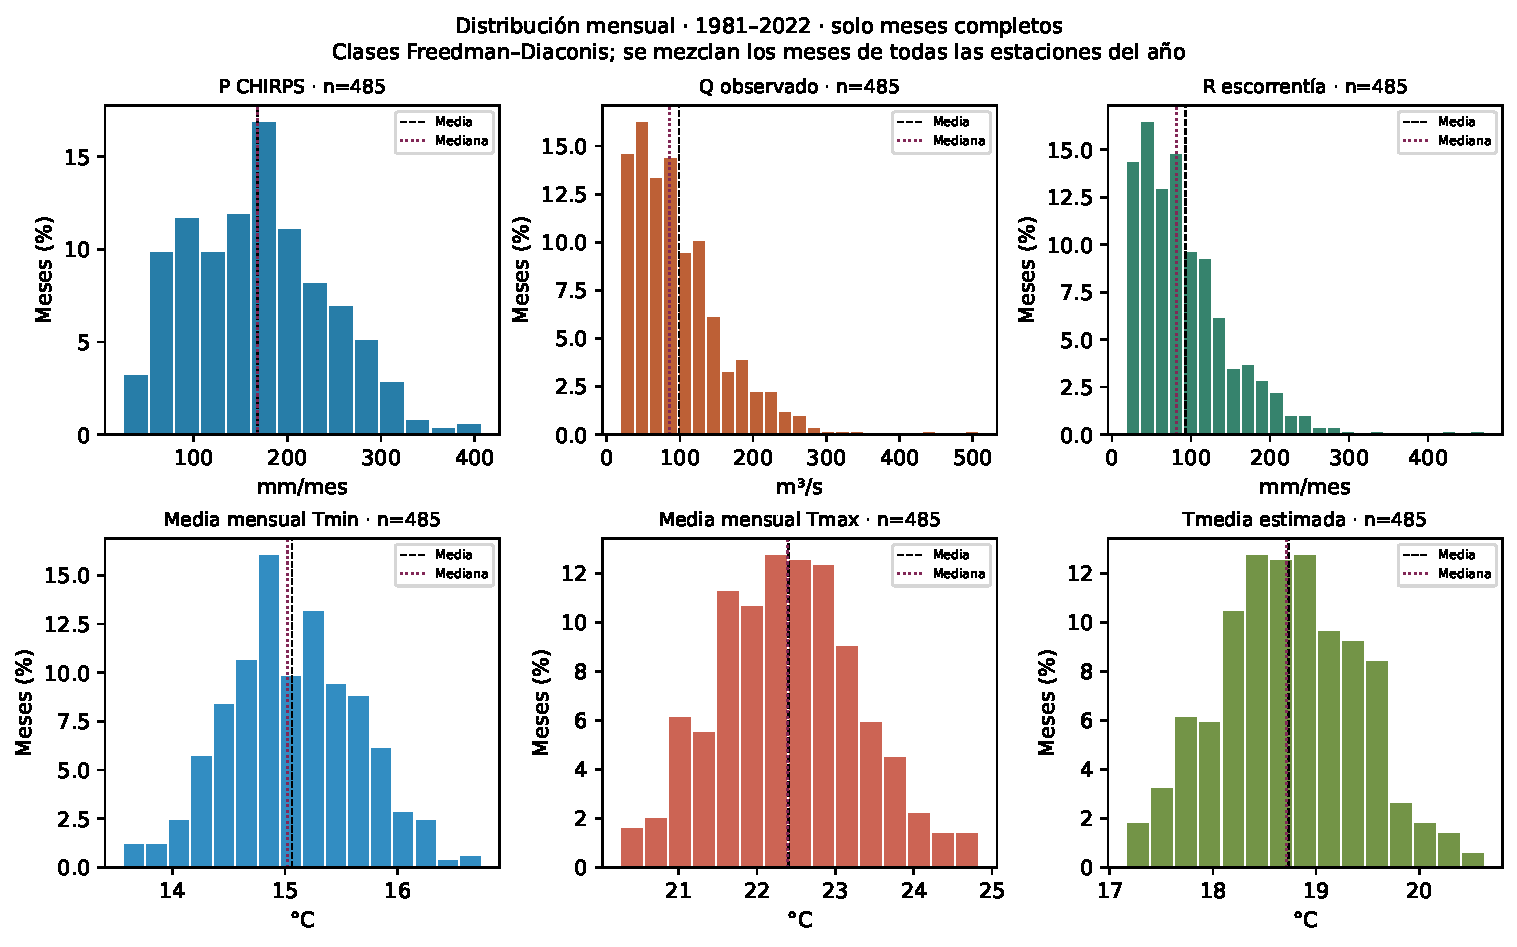
\includegraphics[width=\linewidth]{figuras/histogramas_completos.pdf}
\caption{Distribuciones de meses válidos, 1981--2022; unidades indicadas en cada panel.}
\end{figure}

\subsubsection*{Diagramas de caja}
Se construyen diagramas de caja con los 485 meses completos entre enero de 1981 y diciembre de 2022. Los 19 meses con algún día faltante se excluyen; no se reemplazan por cero. P, Q y R no tienen meses válidos con valor cero. Para temperatura, un valor de 0~$^\circ$C se consideraría una observación válida y nunca una ausencia.

P presenta media y mediana muy próximas (168,20 y 168,47~mm), pero un rango amplio. Q y R muestran media mayor que mediana (98,70 frente a 85,55~m$^3$/s; 92,82 frente a 81,40~mm), consistente con asimetría hacia valores altos y con crecientes poco frecuentes. Los puntos fuera de 1,5 veces el IQR no se eliminan: deben revisarse en las cronologías y, cuando sea posible, contra los datos diarios y metadatos. Las cajas de temperatura son mucho más compactas que las de P, Q y R.

\begin{figure}[H]\centering
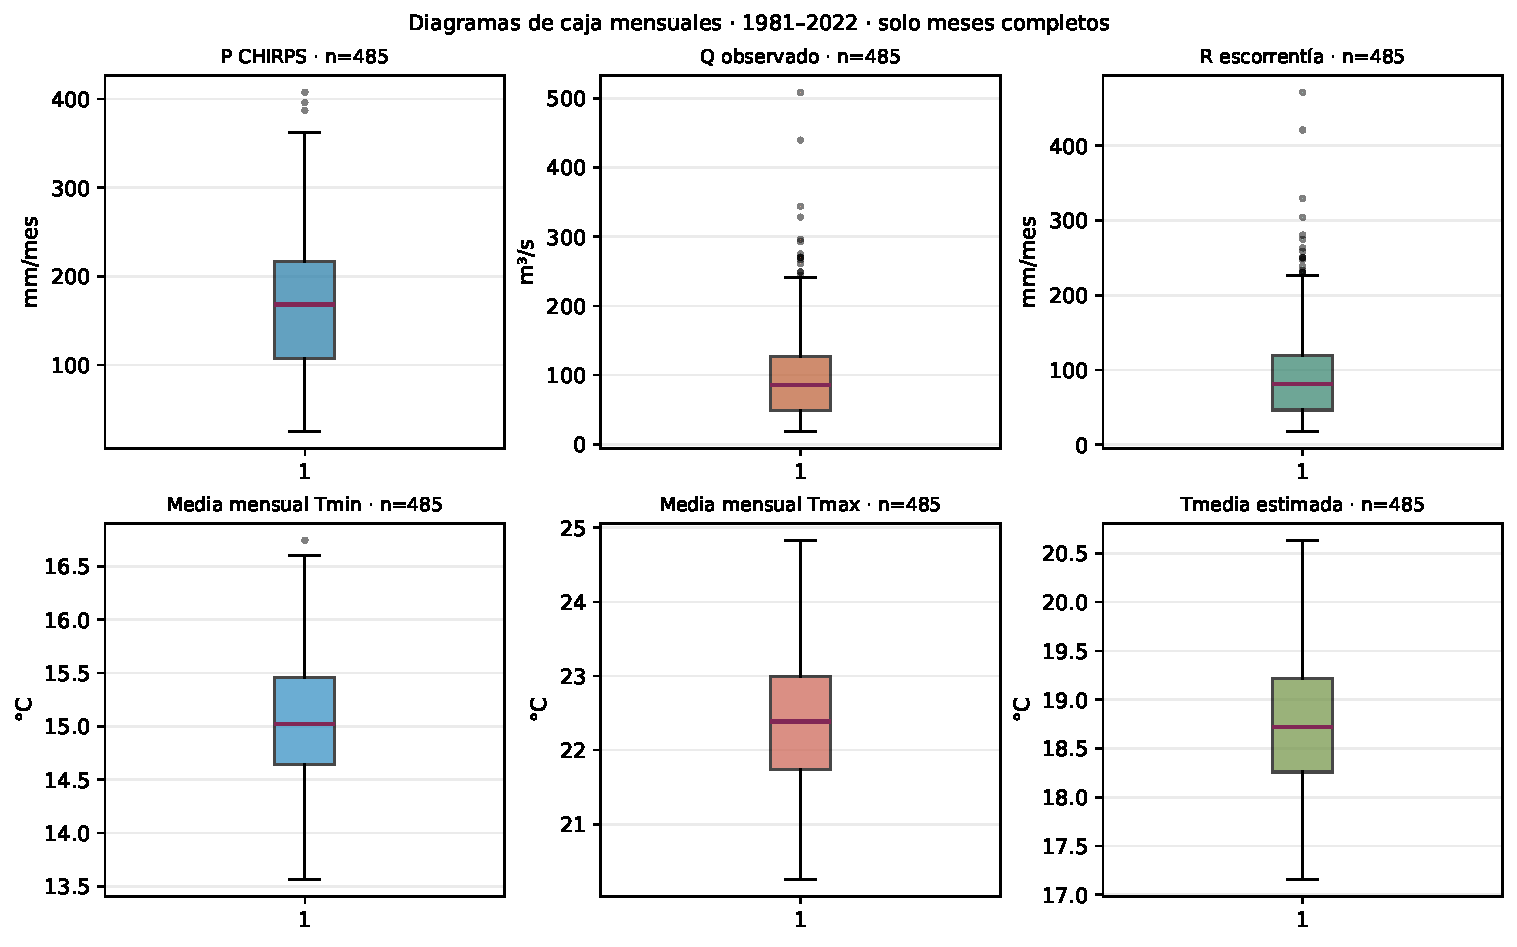
\includegraphics[width=\linewidth]{figuras/diagramas_caja.pdf}
\caption{Diagramas de caja de meses válidos. La línea central es la mediana; la caja representa Q1--Q3; los puntos son valores fuera de 1,5 IQR.}
\end{figure}

\subsubsection*{Cuadrículas comparables: IMERG, Q, R y temperatura}
Esta sección reproduce la estructura de seis paneles de CHIRPS para permitir la comparación visual solicitada. La primera celda usa precipitación IMERG Final Run V07 y las cinco restantes usan Q, R, Tmin, Tmax y Tmedia estimada. Para que las diferencias no se deban a cobertura desigual, todas las variables se calculan sobre los mismos 285 meses completos simultáneos entre enero de 1998 y diciembre de 2022. IMERG conserva el color naranja en sus dos cuadrículas.

El bloque anterior de IMERG con 300 meses sigue siendo útil para comprobar disponibilidad total, pero estas cuadrículas comparables usan solo los 285 meses donde también existe Q. Los histogramas usan clases Freedman--Diaconis y porcentajes de meses. En las cajas, la línea central es la mediana, la caja P25--P75 y el triángulo verde la media.

\begin{figure}[H]\centering
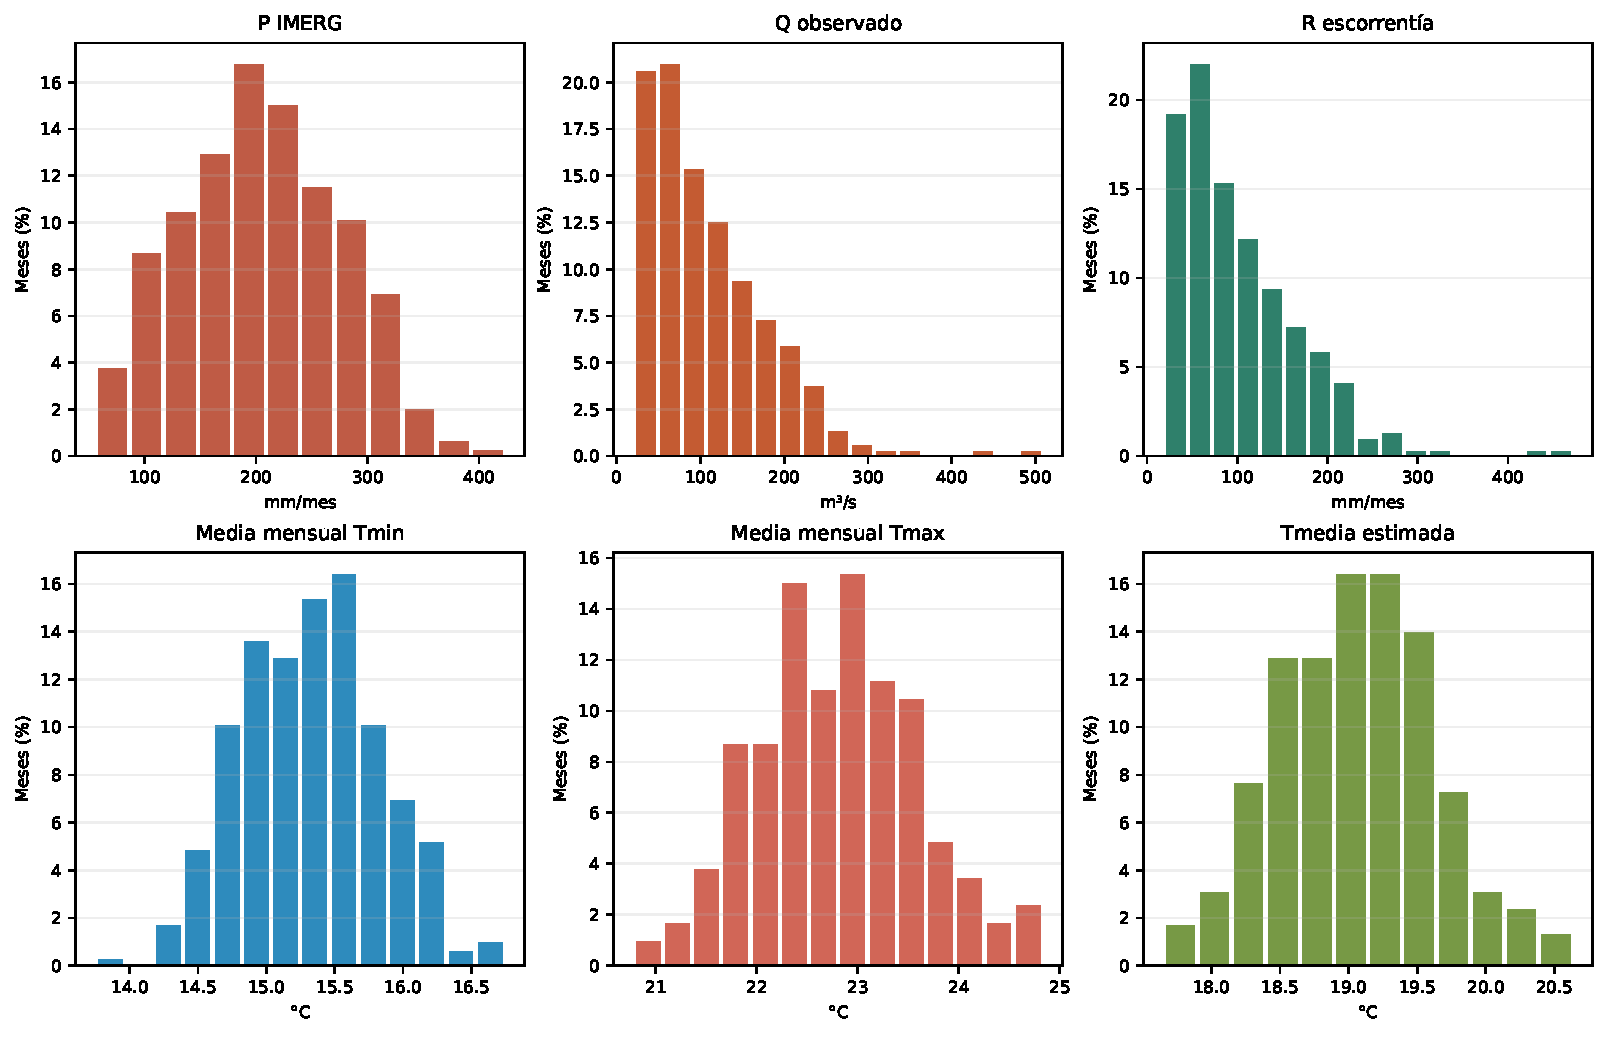
\includegraphics[width=\linewidth]{figuras/imerg_histogramas_comparables.pdf}
\caption{Histogramas comparables del periodo común: IMERG, Q, R, Tmin, Tmax y Tmedia estimada (n=285).}
\end{figure}

\begin{figure}[H]\centering
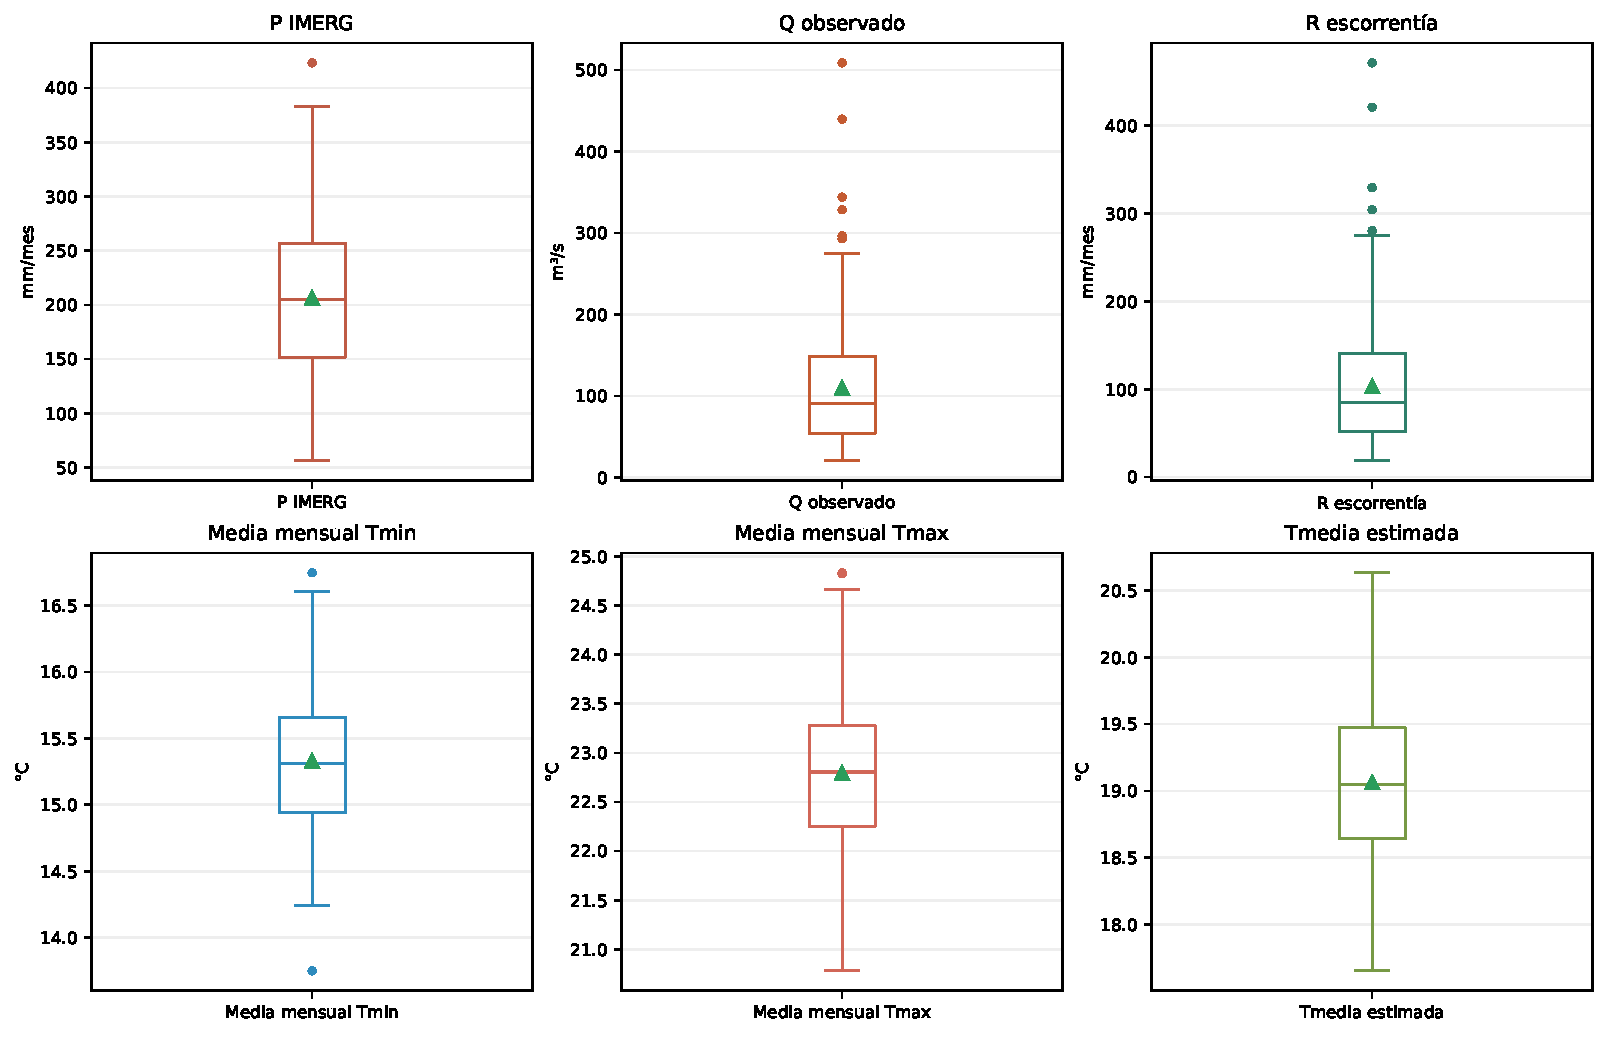
\includegraphics[width=\linewidth]{figuras/imerg_cajas_comparables.pdf}
\caption{Diagramas de caja comparables del mismo periodo común (n=285).}
\end{figure}
\subsubsection*{P (mm/mes), Q (m$^3$/s) y R (mm/mes)}
\begin{center}\small\begin{tabular}{lrrr}\hline
Estadístico & P & Q & R \\ \hline
Meses válidos & 485 & 485 & 485 \\
Media & 168,20 & 98,70 & 92,82 \\
Mediana & 168,47 & 85,55 & 81,40 \\
Desv. estándar & 74,54 & 64,35 & 60,63 \\
Mínimo & 24,89 & 18,37 & 17,59 \\
Máximo & 407,57 & 508,77 & 471,45 \\
Rango & 382,68 & 490,40 & 453,86 \\
Q1 (25\%) & 107,29 & 49,16 & 46,55 \\
Q2 (50\%) & 168,47 & 85,55 & 81,40 \\
Q3 (75\%) & 216,55 & 127,04 & 118,83 \\
IQR & 109,25 & 77,89 & 72,28 \\
P5 & 60,32 & 29,19 & 27,56 \\
P10 & 74,95 & 34,13 & 32,07 \\
P90 & 270,77 & 181,19 & 172,69 \\
P95 & 296,48 & 221,01 & 206,71 \\
Meses con cero & 0 & 0 & 0 \\
\hline\end{tabular}\end{center}
\subsubsection*{Tmin, Tmax y Tmedia estimada ($^\circ$C)}
\begin{center}\small\begin{tabular}{lrrr}\hline
Estadístico & Tmin & Tmax & Tmedia estimada \\ \hline
Meses válidos & 485 & 485 & 485 \\
Media & 15,06 & 22,40 & 18,73 \\
Mediana & 15,02 & 22,39 & 18,72 \\
Desv. estándar & 0,58 & 0,91 & 0,68 \\
Mínimo & 13,56 & 20,25 & 17,16 \\
Máximo & 16,75 & 24,83 & 20,63 \\
Rango & 3,18 & 4,58 & 3,48 \\
Q1 (25\%) & 14,65 & 21,74 & 18,26 \\
Q2 (50\%) & 15,02 & 22,39 & 18,72 \\
Q3 (75\%) & 15,46 & 23,00 & 19,22 \\
IQR & 0,81 & 1,25 & 0,96 \\
P5 & 14,17 & 20,96 & 17,61 \\
P10 & 14,34 & 21,18 & 17,81 \\
P90 & 15,81 & 23,58 & 19,60 \\
P95 & 16,05 & 23,94 & 19,84 \\
Meses con cero & 0 & 0 & 0 \\
\hline\end{tabular}\end{center}
\subsubsection*{Precipitación in situ: existencia y alcance}
Sí existen mediciones terrestres distintas de CHIRPS. El POMCA La Vieja,
capítulo 3, tabla 3.7, documenta registros de Salento (26120160), Alcalá
(26120150), Cumbarco (26125130) y Aeropuerto El Edén (26125060).
Son mediciones puntuales; un promedio de cuenca requiere evaluar periodos,
faltantes, distribución espacial y ponderación. Fuente:
\href{https://www.cvc.gov.co/sites/default/files/Planes_y_Programas/Planes_de_Ordenacion_y_Manejo_de_Cuencas_Hidrografica/La%20Vieja%20-%20POMCA%20en%20Ajuste/Fase%20Diagnostico/3_CapituloI_Diagnostico_Clima.pdf}{POMCA La Vieja, capítulo Clima}.

Las climatologías publicadas no sustituyen una serie cronológica de 25 años.
No se han incorporado registros terrestres sin auditar: los histogramas de
precipitación de este documento corresponden a CHIRPS.
\subsubsection*{IMERG: distribución y control descriptivo}

En este apartado se presentan únicamente serie, distribución, caja y estadísticos de IMERG; no se superponen con CHIRPS. El catálogo identifica 172 instalaciones dentro o en el borde de la cuenca, de las cuales 131 están clasificadas como lluvia. Ese conteo solo indica cobertura potencial: no demuestra continuidad de las series ni que esas estaciones hayan sido usadas como datos de entrada.

\begin{figure}[H]\centering
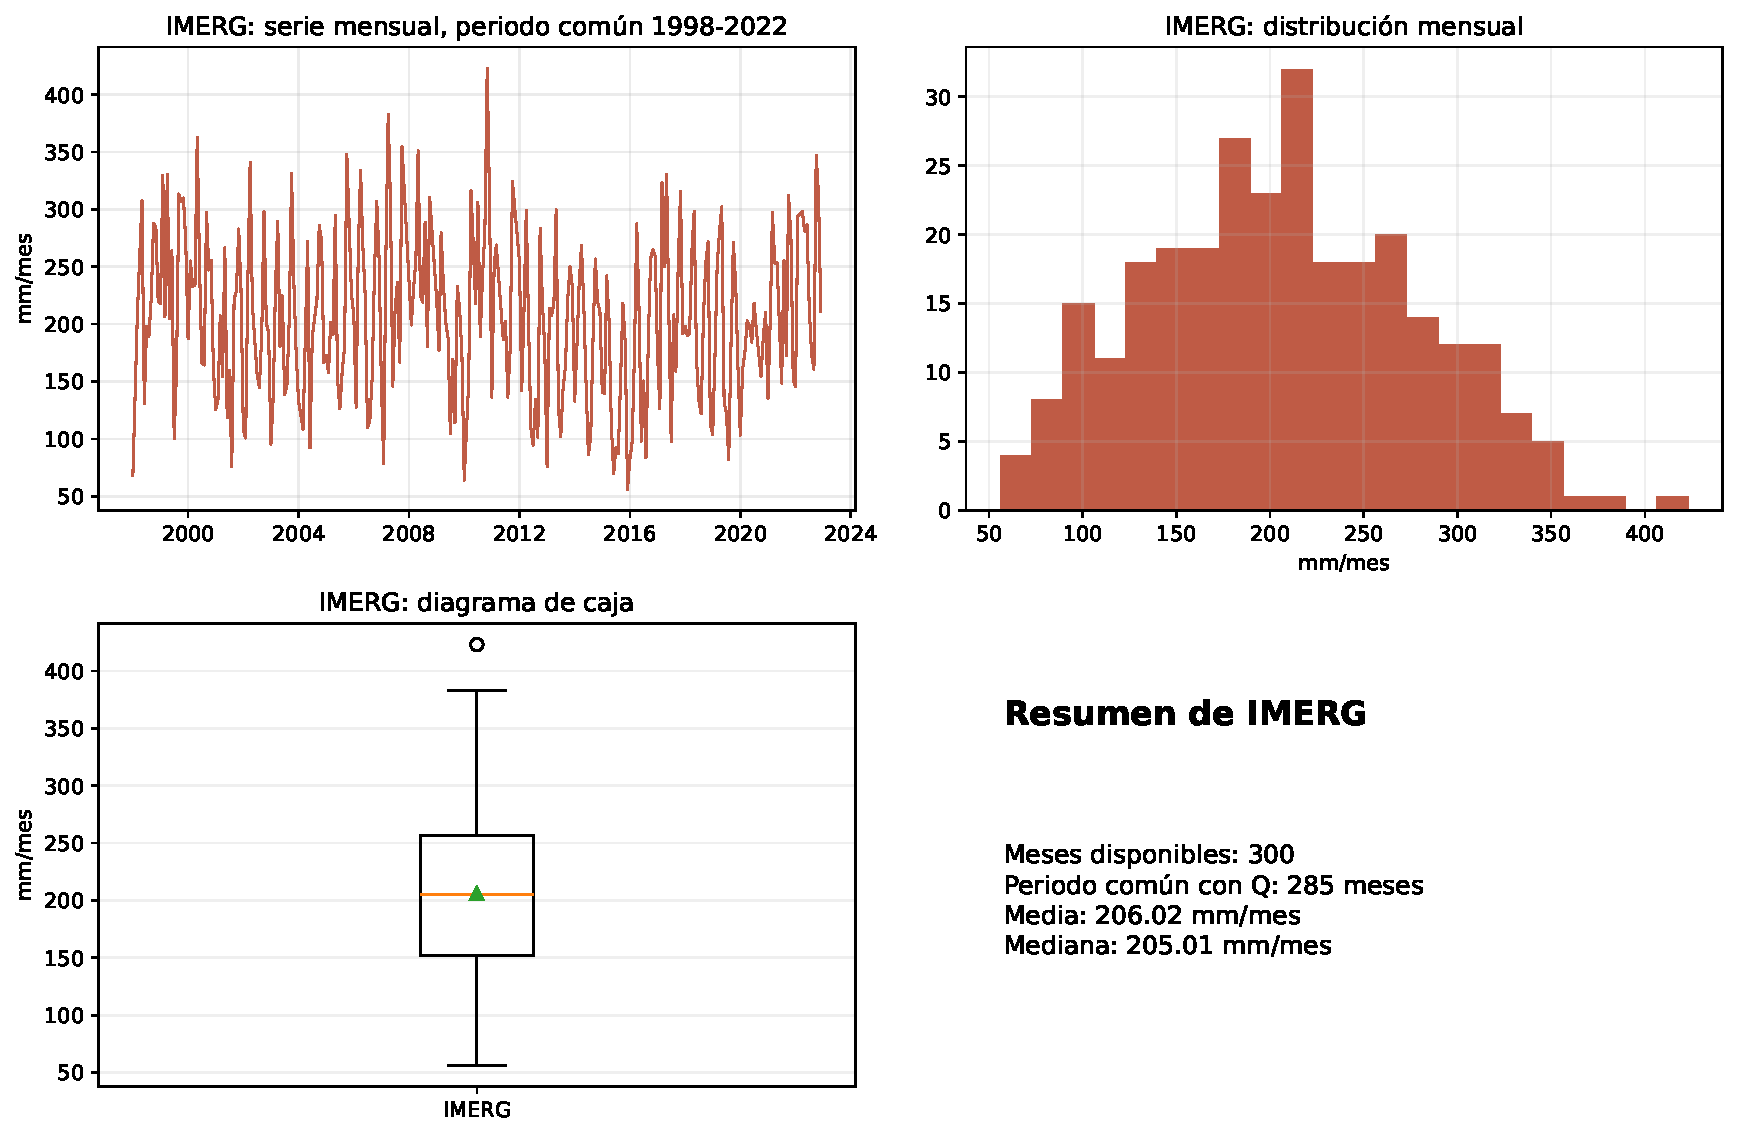
\includegraphics[width=\linewidth]{figuras/imerg_complemento.pdf}
\caption{IMERG incorporado al análisis: serie cronológica, distribución, diagrama de caja y resumen del periodo común.}
\end{figure}



\subsection{Usar la exploración como control de calidad}
\subsubsection*{Control de datos faltantes}
Se reconstruyó el calendario diario completo de 1981--2022, incluidos los años
bisiestos. De 15\,340 días esperados, el archivo contiene 15\,085 fechas y omite
255 días (1,66\,\%) tanto en P como en Q. Son las mismas fechas ausentes para
ambas variables: no se deben sumar como 510 días distintos.

\subsubsection*{Criterio de completitud}
Se retiene únicamente un mes con el 100\,\% de sus días válidos. De 504 meses,
se conservan 485 (96,23\,\%) y se excluyen 19 (3,77\,\%): seis totalmente ausentes
y trece parcialmente completos. Los ceros se conservan y los faltantes permanecen
como vacíos; no se rellena ni se prorratea la precipitación.

\begin{figure}[H]
\centering
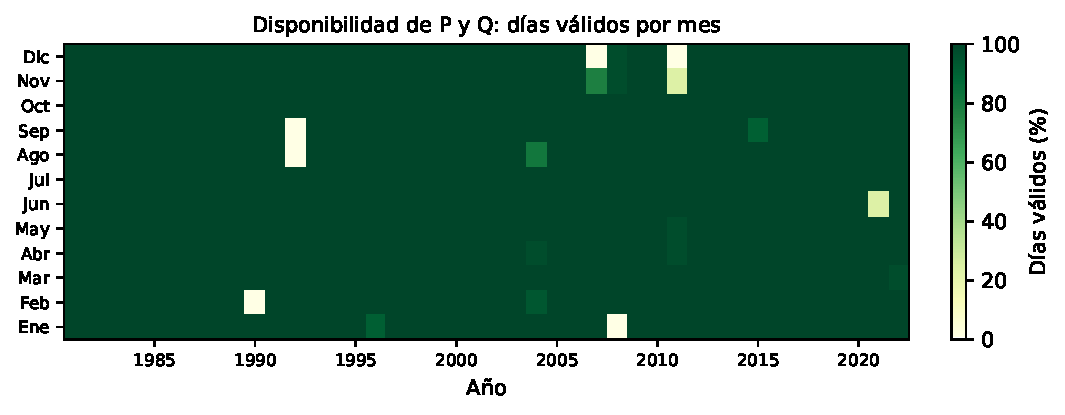
\includegraphics[width=\linewidth]{figuras/control_faltantes.pdf}
\caption{Disponibilidad diaria dentro de cada mes. P y Q tienen la misma cobertura
en el archivo CAMELS; 100\,\% indica un mes completo.}
\label{fig:faltantes}
\end{figure}

\begin{center}
\small
\begin{tabular}{lrrrr}
\hline
Mes & Esperados & Válidos P/Q & Faltantes P/Q & Completitud (\%) \\
\hline
1990-02 & 28 & 0 & 28 & 0,00 \\
1992-08 & 31 & 0 & 31 & 0,00 \\
1992-09 & 30 & 0 & 30 & 0,00 \\
1996-01 & 31 & 28 & 3 & 90,32 \\
2004-02 & 29 & 27 & 2 & 93,10 \\
2004-04 & 30 & 29 & 1 & 96,67 \\
2004-08 & 31 & 25 & 6 & 80,65 \\
2007-11 & 30 & 23 & 7 & 76,67 \\
2007-12 & 31 & 0 & 31 & 0,00 \\
2008-01 & 31 & 0 & 31 & 0,00 \\
2008-11 & 30 & 29 & 1 & 96,67 \\
2008-12 & 31 & 30 & 1 & 96,77 \\
2011-04 & 30 & 29 & 1 & 96,67 \\
2011-05 & 31 & 30 & 1 & 96,77 \\
2011-11 & 30 & 7 & 23 & 23,33 \\
2011-12 & 31 & 0 & 31 & 0,00 \\
2015-09 & 30 & 27 & 3 & 90,00 \\
2021-06 & 30 & 7 & 23 & 23,33 \\
2022-03 & 31 & 30 & 1 & 96,77 \\
\hline
\end{tabular}
\end{center}

\subsubsection*{Consecuencias para la interpretación}
Los vacíos continuos más largos son diciembre de 2007--enero de 2008 (62 días),
agosto--septiembre de 1992 (61 días) y 8 de noviembre--31 de diciembre de 2011
(54 días). No es posible reconstruir su evolución a partir del archivo analizado;
los faltantes pueden sesgar la representación de temporadas y extremos.

Como sensibilidad, aceptar meses de Q con al menos 90\,\% de días elevaría la
muestra a 494 meses y la media a 100,91~m$^3$/s, frente a 98,70~m$^3$/s con el
criterio estricto. Se mantiene el 100\,\% como resultado principal. Esta comparación
no justifica tratar sumas parciales de precipitación como acumulados completos.

Este control describe el archivo CAMELS ensamblado, no la disponibilidad original
de CHIRPS, IMERG ni de las estaciones pluviométricas individuales. No se supone
que los faltantes ocurran al azar.


\subsection{Climatología, variabilidad y explicación física}
\subsubsection*{Lectura temporal con IMERG}
IMERG muestra dos máximos estacionales: abril--mayo (medias de 273,27 y 257,47~mm/mes) y octubre--noviembre (276,25 y 276,03~mm/mes). Los meses medios más secos son enero (144,68), julio (153,95) y agosto (154,74~mm/mes). Este patrón describe el ciclo observado por el producto y no demuestra una causa climática por sí solo.
Apartado pendiente de completar según la guía; esta reorganización no incorpora resultados nuevos.
\subsubsection*{1.5.a. Construir la climatología de doce meses}
Pendiente de completar e integrar.
\subsubsection*{1.5.b. Describir y contrastar el ciclo anual}
Pendiente de completar e integrar.
\subsubsection*{1.5.c. Explicar los procesos regionales y de la cuenca}
Pendiente de completar e integrar.
\clearpage
\section{Relaciones entre series y modelos estadísticos}

\subsection{Diagramas de dispersión e interpretación}
\subsubsection*{Diagramas requeridos con IMERG y lluvia local}
Se construyeron los tres diagramas solicitados: IMERG frente a lluvia local, lluvia local frente a caudal Q e IMERG frente a caudal Q. Los puntos se colorean por mes calendario. La estación Zaragoza-AUT ofrece solo 22 meses simultáneos completos en esta descarga; por eso las dos relaciones que incluyen lluvia local son exploratorias y no representan toda la serie 1998--2022.

\begin{figure}[H]\centering
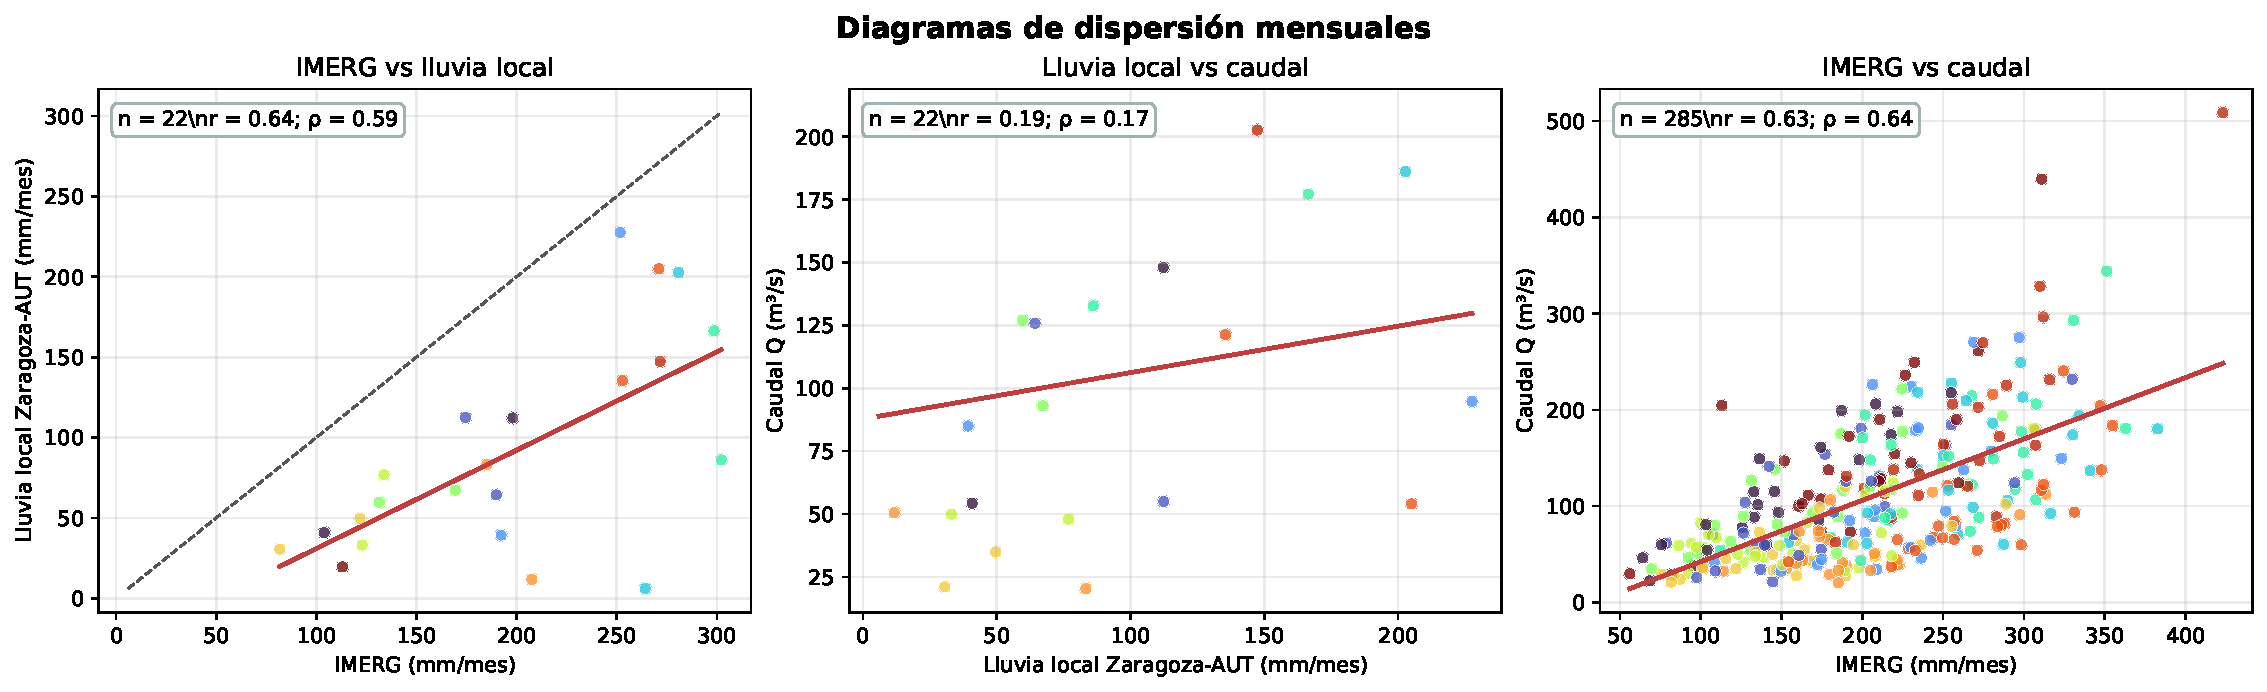
\includegraphics[width=\linewidth]{figuras/dispersiones_requeridas.pdf}
\caption{Diagramas de dispersión requeridos. La línea discontinua en IMERG--lluvia local es 1:1.}
\end{figure}

Para IMERG--lluvia local, Pearson es 0,64 y Spearman 0,59; el sesgo IMERG menos local es +106,42 mm/mes, MAE 106,42 mm/mes y RMSE 120,17 mm/mes. Lluvia local--Q tiene Pearson 0,19 y Spearman 0,17 (n=22); IMERG--Q tiene Pearson 0,63 y Spearman 0,64 (n=285). Son estadísticas descriptivas; falta comparar anomalías mensuales y evaluar rezagos sin usar precipitación futura.

\subsubsection*{Diagramas de dispersión y disponibilidad}
Con los datos disponibles se compara CHIRPS con caudal, usando meses simultáneos
y colores por mes calendario. \textbf{CHIRPS no es una estación de lluvia terrestre.}
\begin{figure}[H]\centering
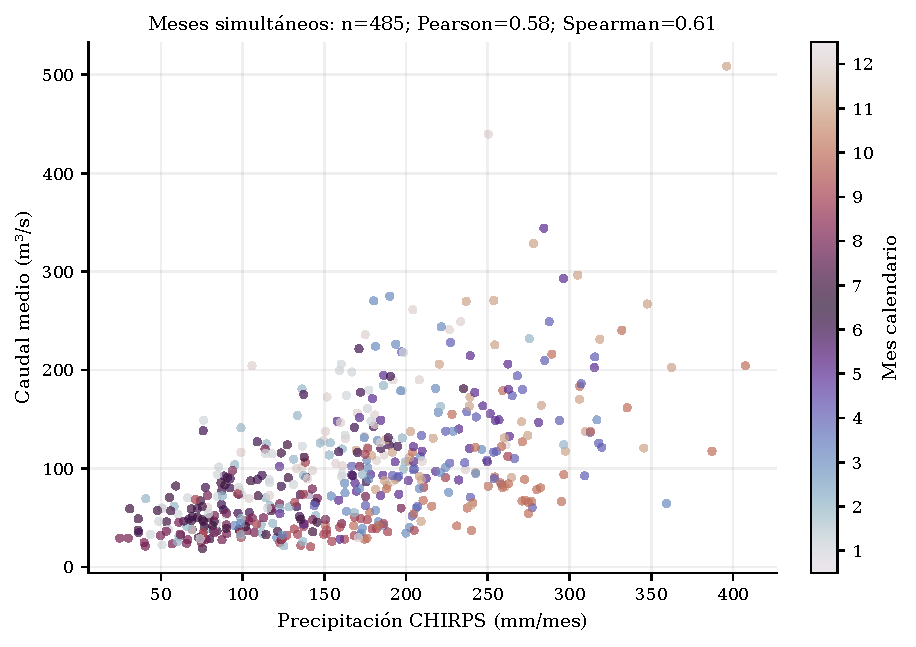
\includegraphics[width=.85\linewidth]{figuras/dispersion_CHIRPS_caudal.pdf}
\caption{Relación descriptiva entre precipitación CHIRPS y caudal, sin rezago.}
\end{figure}
La correlación contiene el ciclo anual compartido y no demuestra causalidad ni
capacidad predictiva. No se evaluó significancia considerando dependencia temporal.
Las comparaciones IMERG--estaciones, estaciones--caudal e IMERG--caudal siguen
pendientes: no se dispone de valores descargados de IMERG ni series terrestres
verificadas. El acceso NASA devolvió HTTP 401 y el grupo indicó que no dispone
de acceso. No se crean puntos ficticios ni se sustituye IMERG por CHIRPS.

\subsubsection*{CHIRPS--Q: análisis paralelo}
Se conservan P CHIRPS acumulada y Q observado de 485 meses completos,
entre enero de 1981 y diciembre de 2022. CHIRPS es una estimación espacial, no
una estación terrestre. Se interpreta en paralelo con IMERG: ninguna de las dos fuentes
sustituye a la otra. Los pares IMERG--lluvia local, IMERG--Q y lluvia local--Q
se presentan arriba; para IMERG aún faltan las comparaciones con anomalías mensuales
y el análisis de rezagos.

\begin{figure}[H]\centering
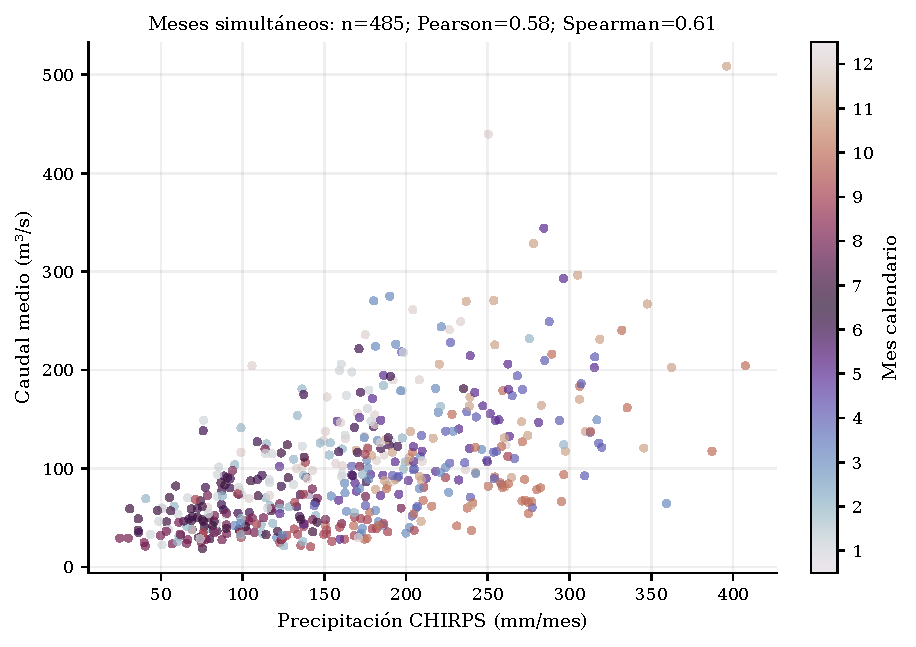
\includegraphics[width=.85\linewidth]{figuras/dispersion_CHIRPS_caudal.pdf}
\caption{Dispersión de P CHIRPS y Q observado. El color identifica el mes calendario.}
\end{figure}

Con valores mensuales Pearson es 0,58 y Spearman es 0,61. Parte de la asociación puede provenir del ciclo anual común. Al quitar el promedio histórico de cada mes calendario, Pearson es 0,56 y Spearman es 0,58. Las anomalías responden mejor a si un mes más lluvioso de lo habitual coincide con caudal mayor de lo habitual.

\begin{center}\small\begin{tabular}{rrrr}\hline
Rezago P (meses) & Meses emparejados & Pearson & Spearman \\ \hline
0 & 485 & 0,58 & 0,61 \\
1 & 484 & 0,61 & 0,68 \\
2 & 483 & 0,27 & 0,33 \\
3 & 482 & -0,06 & -0,07 \\
\hline\end{tabular}\end{center}
El mayor Pearson a escala mensual se observa con P rezagada 1 mes(es) (0,61). Esto no demuestra un tiempo físico de respuesta: los promedios mensuales pueden ocultar respuestas de días/semanas y Q depende además de humedad antecedente, almacenamiento y operación.

No se reportan p-valores simples porque los meses consecutivos son dependientes. Estas correlaciones no prueban causalidad ni son un modelo de pronóstico; se requieren rezagos diarios, validación temporal y otras variables.

\subsection{¿Se pueden construir modelos útiles?}
Pendiente de desarrollar.
\subsection{Evaluar fuera del periodo de ajuste}
Pendiente de desarrollar.
\clearpage
\section{Tendencias hidroclimáticas y sus posibles causas}
\subsection{Temperatura y periodos de análisis}
Pendiente de completar e integrar; los resultados existentes se conservan en el apartado 3.4 y las series en el punto 1.
\subsection{Series originales, anomalías y anomalías estandarizadas}
Pendiente de completar e integrar; los resultados existentes se conservan en el apartado 3.4 y las series en el punto 1.
\subsection{Dos escalas de evaluación temporal}
Pendiente de completar e integrar; los resultados existentes se conservan en el apartado 3.4 y las series en el punto 1.
\subsection{Métodos y comparación de resultados}
\subsubsection*{Tendencias temporales}
Se analizaron los 485 meses completos de enero de 1981 a diciembre de 2022.
Para separar la estacionalidad del cambio de largo plazo se usaron anomalías
mensuales: a cada valor se le resta la media histórica de su mes calendario.
Por eso una anomalía positiva significa que el mes estuvo por encima de lo
habitual para ese mes, no que el valor absoluto sea necesariamente alto.

La línea de la figura es una regresión OLS sobre las anomalías. Como resumen
robusto se calculó la pendiente de Sen estacional, comparando únicamente meses
del mismo calendario (eneros entre sí, febreros entre sí, etc.). Mann--Kendall
estacional contrasta una tendencia monotónica; se reporta p bilateral y se toma
$p<0.05$ como evidencia al nivel 5\%. Estos análisis no prueban causalidad ni
resuelven autocorrelación, cambios de estación, regulación, uso del suelo o
falta de homogeneidad del registro.

\begin{figure}[H]\centering
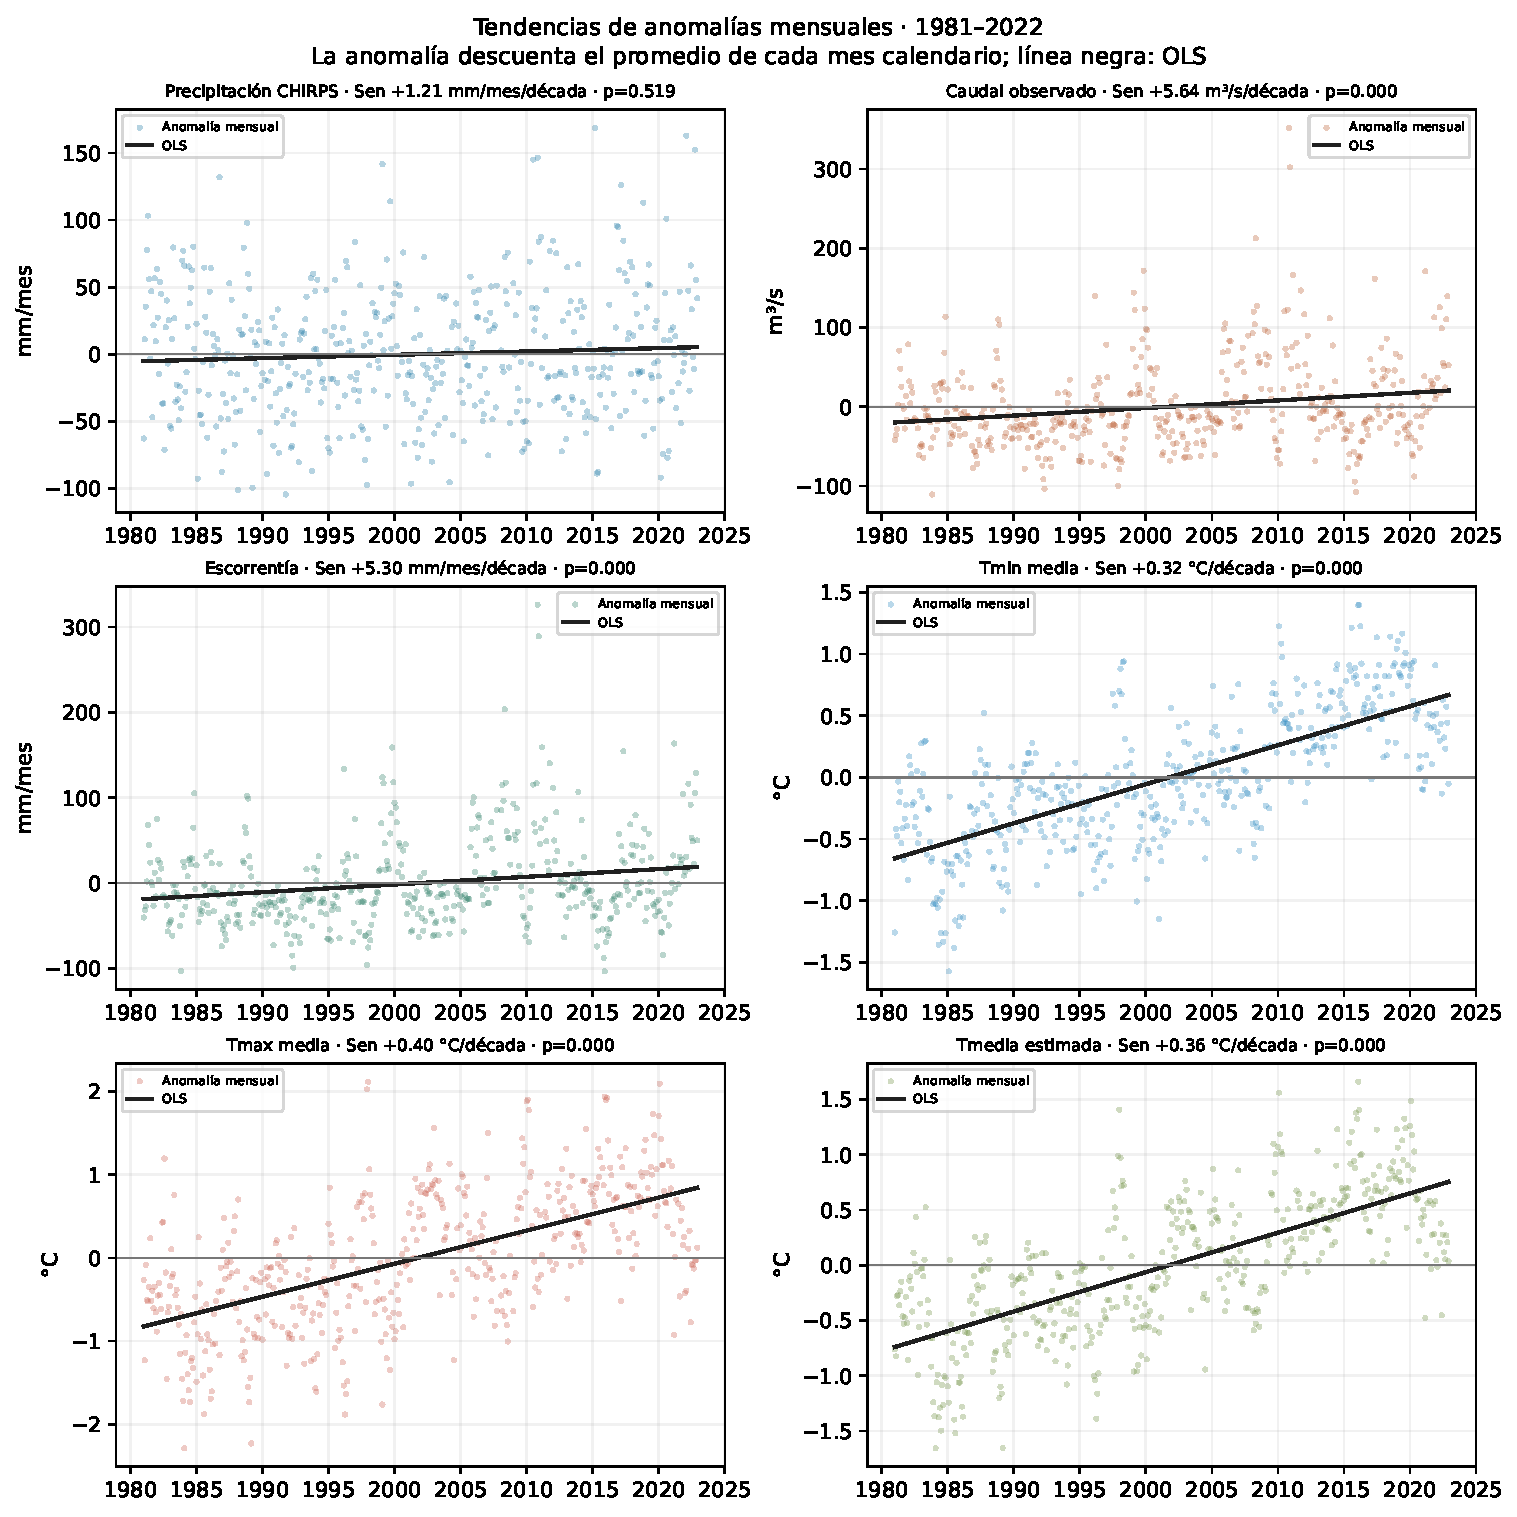
\includegraphics[width=\linewidth]{figuras/tendencias_mensuales.pdf}
\caption{Anomalías mensuales y recta OLS, 1981--2022. Los títulos presentan la pendiente de Sen estacional por década y el valor p de Mann--Kendall estacional.}
\end{figure}

\begin{center}\small
\begin{tabular}{lrrrr}\hline
Variable & OLS/década & Sen/década & p & Significativa 5\% \\ \hline
Precipitación CHIRPS & 2,50 & 1,21 & 0,519 & no \\
Caudal observado & 9,59 & 5,64 & 0,000 & sí \\
Escorrentía & 9,02 & 5,30 & 0,000 & sí \\
Tmin media & 0,32 & 0,32 & 0,000 & sí \\
Tmax media & 0,40 & 0,40 & 0,000 & sí \\
Tmedia estimada & 0,36 & 0,36 & 0,000 & sí \\
\hline\end{tabular}
\end{center}

\subsubsection*{Lectura de los resultados}
\begin{itemize}
\item Precipitación CHIRPS: Sen estacional 1,21 mm/mes/década; p=0,519. no hay evidencia estadística de una tendencia monotónica al 5 \% (aumento).
\item Caudal observado: Sen estacional 5,64 m$^3$/s/década; p=0,000. hay evidencia estadística de una tendencia monotónica al 5 \% (aumento).
\item Escorrentía: Sen estacional 5,30 mm/mes/década; p=0,000. hay evidencia estadística de una tendencia monotónica al 5 \% (aumento).
\item Tmin media: Sen estacional 0,32 $^\circ$C/década; p=0,000. hay evidencia estadística de una tendencia monotónica al 5 \% (aumento).
\item Tmax media: Sen estacional 0,40 $^\circ$C/década; p=0,000. hay evidencia estadística de una tendencia monotónica al 5 \% (aumento).
\item Tmedia estimada: Sen estacional 0,36 $^\circ$C/década; p=0,000. hay evidencia estadística de una tendencia monotónica al 5 \% (aumento).
\end{itemize}
R se deriva directamente de Q, por lo que sus resultados no son evidencias
independientes. Tmedia se estima como $(Tmin+Tmax)/2$ y tampoco es una
observación independiente. IMERG no entra al análisis: aún no se cuenta con
valores mensuales descargados y verificados.
\subsection{Incertidumbre, robustez y presentación}
Pendiente de completar e integrar; los resultados existentes se conservan en el apartado 3.4 y las series en el punto 1.
\subsection{¿A qué podrían deberse los cambios?}
Pendiente de completar e integrar; los resultados existentes se conservan en el apartado 3.4 y las series en el punto 1.
\clearpage
\section{Análisis de frecuencias mediante Fourier}
\subsection{Preparar las series y documentar el cálculo}
Pendiente de desarrollar.
\subsection{Construir e interpretar los espectros}
Pendiente de desarrollar.
\clearpage
\section{Mapas de correlación con el clima global}
\subsection{Seleccionar los campos climáticos}
Pendiente de desarrollar.
\subsection{Definir y calcular los mapas mensuales}
Pendiente de desarrollar.
\subsection{Robustez y presentación de los patrones}
Pendiente de desarrollar.
\subsection{Interpretación física e integración}
Pendiente de desarrollar.
\section*{Conclusiones}
Pendiente de síntesis final.

\section*{Procedencia, alcance y reproducibilidad}
\subsubsection*{Procedencia y alcance}
\subsubsection*{Procedencia de los datos}
Se utiliza CAMELS-COL, depósito del 26 de febrero de 2026, DOI
\href{https://doi.org/10.5281/zenodo.18794895}{10.5281/zenodo.18794895}, consultado
el 21 de septiembre de 2026. El archivo de entrada es
\path{Hydromet_data_26127040.txt}, incluido en
\path{04_CAMELS_COL_Hydrometeorological_data.zip}, para la cuenca del río
La Vieja hasta la estación Cartago (IDEAM 26127040).
\begin{itemize}
\item \textbf{Precipitación:} CHIRPS v2, datos diarios promediados sobre la cuenca
por los autores de CAMELS-COL, en mm/día. Es un producto combinado, no una
medición directa de un único pluviómetro.
\item \textbf{Caudal:} valores diarios reportados como observados en la estación
hidrométrica IDEAM, distribuidos mediante CAMELS-COL, en m$^3$/s. No se
descargaron aforos originales directamente del IDEAM.
\item \textbf{Área y delimitación:} atributos y polígono CAMELS-COL; área
reportada de 2797,19 km$^2$. Nombre y ubicación contrastados con el catálogo IDEAM.
\item \textbf{Temperatura:} el archivo contiene Tmin y Tmax de MSWX; se grafican sus medias mensuales y una Tmedia estimada como $(Tmin+Tmax)/2$, no una media horaria observada.
\end{itemize}

\subsubsection*{Alcance temporal y procesamiento}
Se analiza enero de 1981 a diciembre de 2022 (42 años). Se reconstruyó el
calendario diario y se conservaron solo meses con el 100\,\% de días válidos:
485 de 504 meses. P mensual es la suma de P diaria; Q mensual es la media de Q
diaria. No se rellenaron faltantes, no se prorratearon sumas ni se eliminaron
extremos por su magnitud.

Las estadísticas globales y por año describen valores mensuales válidos. Mínimo
y máximo no son extremos instantáneos ni diarios. La desviación estándar es
muestral. Los años incompletos describen únicamente su muestra disponible.

\subsubsection*{Limitaciones y trabajo pendiente}
Este documento es una exploración descriptiva inicial. La cartografía de relieve utiliza Copernicus GLO-30, documentado en la sección de mapas. Las gráficas no prueban
tendencias, causalidad ni capacidad predictiva. No se ha certificado la
homogeneidad del registro, la ausencia de reconstrucciones previas o el efecto de
extracciones y regulación. No hay banderas por observación en el archivo diario
que permitan resolver esas cuestiones.

\textbf{IMERG está incorporado como promedio de caja para 1998--2022:} falta
calcular el promedio exacto ponderado por fracción de área del polígono y validar
los valores por celda. También quedan pendientes una temperatura media de fuente
directa y los registros individuales de estaciones de lluvia. El conteo de estaciones
no demuestra continuidad de sus series ni significa que se hayan utilizado como datos de entrada.

\subsubsection*{Reproducibilidad y apoyo de IA}
Los scripts numerados se conservan en \path{seleccion_cuenca/scripts/}.
La tabla común a las gráficas es \path{datos_graficados.csv};
\path{proveniencia.json} registra su huella SHA-256 y versiones de bibliotecas.
Las comprobaciones e intermedios están en \path{la_vieja/punto_1/}.
La IA apoyó la programación, la revisión aritmética y la redacción preliminar;
el grupo debe revisar fuentes, decisiones e interpretación.

PDF y HTML representan los mismos datos. El HTML incluye Plotly y las series y
funciona sin servidor ni Internet; consultar fuentes externas sí requiere conexión.

\section*{Uso de IA}
La declaración existente se conserva en el apartado anterior; falta completar la declaración final del grupo.
\section*{Referencias y anexos}
Las referencias y fuentes existentes se conservan junto a sus análisis; falta consolidar el listado final.
\end{document}
